\documentclass[11pt,twoside,a4paper]{book}
\usepackage[utf8]{inputenc}
\usepackage[T1]{fontenc}
\usepackage{latexsym}

\usepackage[brazil,brazilian]{babel}
\usepackage[pdftex]{graphicx}           
\usepackage{setspace}                   
\usepackage{indentfirst}                
\usepackage{makeidx}                  
\usepackage[nottoc]{tocbibind}     
\usepackage{courier}                    
\usepackage{type1cm}              
\usepackage{listings}                   
\usepackage{titletoc}
\usepackage{amsmath}
\usepackage[fixlanguage]{babelbib}
\usepackage[font=small,format=plain,labelfont=bf,up,textfont=it,up]{caption}
\usepackage[usenames,svgnames,dvipsnames]{xcolor}
\usepackage[a4paper,top=2.54cm,bottom=2.0cm,left=2.0cm,right=2.54cm]{geometry} % margens
\usepackage[pdftex,plainpages=false,pdfpagelabels,pagebackref,colorlinks=true,citecolor=DarkGreen,linkcolor=NavyBlue,urlcolor=DarkRed,filecolor=green,bookmarksopen=true]{hyperref} % links coloridos
\usepackage[all]{hypcap}                % soluciona o problema com o hyperref e capitulos
\usepackage[square,sort,nonamebreak,comma]{natbib}  
% \usepackage[chapter]{algorithm}
% \usepackage{algpseudocode}
\usepackage[algochapter,boxruled,linesnumbered,portuguese]{algorithm2e}
\fontsize{60}{62}\usefont{OT1}{cmr}{m}{n}{\selectfont}
\usepackage{fancyhdr}
\usepackage{multirow}
\usepackage{siunitx}
\pagestyle{fancy}
\fancyhf{}
\renewcommand{\chaptermark}[1]{\markboth{\MakeUppercase{#1}}{}}
\renewcommand{\sectionmark}[1]{\markright{\MakeUppercase{#1}}{}}
\renewcommand{\headrulewidth}{0pt}
\renewcommand*{\lstlistingname}{Listagem}
%\renewcommand*{\lstlistoflistingname}{Lista de Listagens}
\graphicspath{{imagens/}}             
\frenchspacing                          
\urlstyle{same}                         
\makeindex                              
\raggedbottom                           
\fontsize{60}{62}\usefont{OT1}{cmr}{m}{n}{\selectfont}
\cleardoublepage
\normalsize
% Ref: http://en.wikibooks.org/wiki/LaTeX/Packages/Listings
\lstset{ %
language=Java,                  % choose the language of the code
basicstyle=\footnotesize,       % the size of the fonts that are used for the code
numbers=left,                   % where to put the line-numbers
numberstyle=\footnotesize,      % the size of the fonts that are used for the line-numbers
stepnumber=1,                   % the step between two line-numbers. If it's 1 each line will be numbered
numbersep=5pt,                  % how far the line-numbers are from the code
showspaces=false,               % show spaces adding particular underscores
showstringspaces=false,         % underline spaces within strings
showtabs=false,                 % show tabs within strings adding particular underscores
frame=single,	                % adds a frame around the code
framerule=0.6pt,
tabsize=2,	                    % sets default tabsize to 2 spaces
captionpos=b,                   % sets the caption-position to bottom
breaklines=true,                % sets automatic line breaking
breakatwhitespace=false,        % sets if automatic breaks should only happen at whitespace
escapeinside={\%*}{*)},         % if you want to add a comment within your code
backgroundcolor=\color[rgb]{1.0,1.0,1.0}, % choose the background color.
rulecolor=\color[rgb]{0.8,0.8,0.8},
extendedchars=true,
xleftmargin=10pt,
xrightmargin=10pt,
framexleftmargin=10pt,
framexrightmargin=10pt
}

% Corpo do texto
\begin{document}
\frontmatter 
\fancyhead[RO]{{\footnotesize\rightmark}\hspace{2em}\thepage}
\setcounter{tocdepth}{2}
\fancyhead[LE]{\thepage\hspace{2em}\footnotesize{\leftmark}}
\fancyhead[RE,LO]{}
\fancyhead[RO]{{\footnotesize\rightmark}\hspace{2em}\thepage}

\onehalfspacing

% ---------------------------------------------------------------------------- %
% CAPA
% Nota: O título para as dissertações/teses do IME-USP devem caber em um 
% orifício de 10,7cm de largura x 6,0cm de altura que há na capa fornecida pela SPG.
\thispagestyle{empty}
\begin{center}
    \vspace*{2.3cm}
    \textbf{\Large{Uma infraestrutura para desenvolvimento de aplicações distribuídas baseada em minitransações}}\\
    
    \vspace*{1.2cm}
    \Large{Leandro Ferro Luzia}
    
    \vskip 2cm
    \textsc{
    Dissertação apresentada\\[-0.25cm] 
    ao\\[-0.25cm]
    Instituto de Matemática e Estatística\\[-0.25cm]
    da\\[-0.25cm]
    Universidade de São Paulo\\[-0.25cm]
    para\\[-0.25cm]
    obtenção do título\\[-0.25cm]
    de\\[-0.25cm]
    Mestre em Ciências}
    
    \vskip 1.5cm
    Programa: Ciências da Computação\\
    Orientador: Prof. Dr. Francisco C. R. Reverbel
    \vskip 1cm
    
    \vskip 0.5cm
    \normalsize{São Paulo, Junho de 2013}
\end{center}

% ---------------------------------------------------------------------------- %
% Página de rosto (SÓ PARA A VERSÃO DEPOSITADA - ANTES DA DEFESA)
% Resolução CoPGr 5890 (20/12/2010)
\newpage
\thispagestyle{empty}
    \begin{center}
        \vspace*{2.3 cm}
        \textbf{\Large{Uma infraestrutura para desenvolvimento de aplicações distribuídas baseada em minitransações}}\\
        \vspace*{2 cm}
    \end{center}

    \vskip 2cm

    \begin{flushright}
	Esta é a versão original da dissertação elaborada pelo\\
	candidato Leandro Ferro Luzia, tal como \\
	submetida à Comissão Julgadora.
    \end{flushright}

\pagebreak

\pagenumbering{roman}

%\chapter*{Agradecimentos}
%Texto texto texto texto texto texto texto texto texto texto texto texto texto
%texto texto texto texto texto texto texto texto texto texto texto texto texto
%texto texto texto texto texto texto texto texto texto texto texto texto texto
%texto texto texto texto. Texto opcional.

\chapter*{Resumo}

\noindent LUZIA, L. F. \textbf{Uma infraestrutura para desenvolvimento de aplicações distribuídas baseada em minitransações}. 
2012. 120 f.
Dissertação (Mestrado) - Instituto de Matemática e Estatística,
Universidade de São Paulo, São Paulo, 2013.
\\

Resumo...
%Este trabalho apresenta uma infraestrutura para sistemas distribuídos que oferece uma abstração de estado compartilhado entre as máquinas na forma de um repositório de dados utilizando minitransações para garantir a atomicidade na execução de grupos de operações sobre esse repositório. As minitransações são uma modificação do protocolo de efetivação em duas fases em que todas as operações que compõem a transação são enviadas de uma só vez, diminuindo o custo de comunicação entre as máquinas do sistema. Com o uso da primitiva de minitransação os desenvolvedores podem projetar sistemas distribuídos baseando o compartilhamento de estado entre as máquinas em estruturas de dados, e não na troca explícita de mensagens. As máquinas terão à disposição um repositório de dados que pode crescer de forma a acomodar grandes quantidades de dados e que permite que aplicações tenham sempre acesso a dados consistentes. Assim, esperamos que o desenvolvimento da aplicação distribuída seja mais simples e ajude o desenvolvedor a focar nas necessidades reais da aplicação.
\\

\noindent \textbf{Palavras-chave:} minitransação, transação, banco de dado, sistemas distribuídos.

\chapter*{Abstract}
\noindent LUZIA, L. F. \textbf{An infrastructure for developing distributed applications based in minitransactions}. 
2010. 120 f.
Dissertação (Mestrado) - Instituto de Matemática e Estatística,
Universidade de São Paulo, São Paulo, 2013.
\\
TODO reescrever por que alterei o resumo em português

In this work, we propose an infrastructure for distributed systems that allows
state sharing abstraction among machines as a data repository using minitransactions to ensure atomicity when executing groups of operations over 
this repository. Minitransactions are a modification in the two phase 
commit protocol such that all transaction operations are sent in one network round trip, reducing the overhead of communication. By using the 
minitransaction primitive developers can design distributed systems in which the state sharing is based in the usage of data structures and not 
explicit message exchange. The machines will have access to a data repository that can grow to serve large amounts of data and allow applications 
to access consistent data. This way, we expect to facilitate the development of
distributed applications and to help developers to focus in the real needs of
the applications.
\\

\noindent \textbf{Keywords:} minitransaction, transaction, database, distributed systems.

\tableofcontents

% \chapter{Lista de Abreviaturas}
% \begin{tabular}{ll}
% 	ACID    & Atomicidade, Consistência, Isolamento e Durabilidade \\
%             & (\emph{Atomicity, Consistency, Isolation and Durability})\\
%     SGBD	& Sistema Gerenciador de Banco de Dados\\
% 	2PC		& Efetivação em Duas Fases (\emph{Two-Phase Commit})\\
% 	TCP/IP	& Conjunto de protocolos de comunicação utilizado na Internet\\
% 			& (\emph{Transmition Control Protocol} e \emph{Internet Protocol})\\
% \end{tabular}

\listoffigures
\listoftables
\listofalgorithms
\lstlistoflistings
\mainmatter

% cabeçalho para as páginas de todos os capítulos
\fancyhead[RE,LO]{\thesection}

\singlespacing              % espaçamento simples

\chapter{Introdução}
\label{chap:introducao}
%Há diversos motivos para construirmos uma aplicação de forma distribuída, como por exemplo o compartilhamento de recursos, tolerância a falhas e escalabilidade, mas desenvolver um sistema distribuído com essas características não é uma tarefa simples nem trivial. 

%Múltiplos fatores fazem com que o desenvolvimento de aplicações distribuídas exija um esforço adicional em relação ao necessário para construir sistemas  convencionais. Dentre esses fatores podemos mencionar diferentes plataformas de hardware, diferentes sistemas operacionais, comunicação não síncrona entre as máquinas, e falhas e conhecimento parcial do sistema.

Um sistema distribuído é uma coleção de dispositivos computacionais individuais que podem se comunicar uns com os outros \cite{tanenbaum, distributed_computing}. Essa definição engloba uma gama de sistemas computacionais atuais, desde placas de circuitos integrados contendo diversos processadores até a \emph{Internet}. 

Os sistemas distribuídos aos quais este trabalho se refere são compostos por diversos computadores interligados por uma rede de comunicação. Cada computador nesses sistemas possui acesso somente ao seu próprio sistema de armazenamento e a única forma de compartilhar informação é por meio da troca de dados pela rede de comunicação.

Como exemplos podemos citar desde sistemas clássicos como o serviço de nomes de domínio da internet (\emph{DNS}, ou \emph{Domain Name Service}, que mapeia nomes de domínios para endereços de rede \cite{dns}), o correio eletrônico (\emph{email} \cite{email}) e a rede de alcance global (\emph{WWW}, ou \emph{World Wide Web} \cite{www}); passando por sistemas de compartilhamento de dados e de comunicação diretamente entre usuários, os chamados sistemas ponto-a-ponto, como \emph{Skype}, \emph{BitTorrent} e \emph{Gnutella}, sistemas de busca como \emph{Google} ou \emph{Bing} e redes sociais como \emph{Facebook} ou \emph{Twitter}; até jogos online com número maciço de jogadores(\emph{MMOG}, ou \emph{Massive Multiplayer Online Game}) e dinheiro eletrônico (\emph{BitCoin} \cite{bitcoin}).

A implementação de sistemas distribuídos em larga escala é complexa, pois esses sistemas precisam lidar e se recuperar de falhas, controlar e gerenciar o acesso e modificação concorrente do estado do sistema, detectar e corrigir possíveis conflitos que esse acesso concorrente possa causar, tudo isso evitando que o sistema fique indisponível ou que o estado do sistema seja perdido.

Diversas técnicas e mecanismos são utilizados para atingir os objetivos descritos acima, de forma que os usuários possam utilizar esses sistemas de maneira consistente. Aos usuários é exposto um conceito ao mesmo tempo simples e poderoso: transação. Uma transação permite que operações no sistema sejam consideradas como uma única operação lógica, e encapsulam toda a complexidade envolvendo as ações que precisam ser executadas para que essa operação lógica seja bem sucedida.   

%Implementar o compartilhamento de estado da aplicação utilizando a troca de dados na rede não é trivial, em especial quando os dados possuem restrições semânticas que precisam ser mantidas e validadas. Por exemplo, se considerarmos um sistema bancário em que as contas dos usuários estão distribuídas entre diversas máquinas e que temos uma solicitação de transferência entre contas que estão em duas máquinas diferentes, é esperado que essa transferência subtraia uma certa quantia da conta de origem e adicione essa mesma quantia na conta de destino, sem alterar o valor total das contas envolvidas. Se a máquina que armazena os dados da conta de destino falhar, a quantia subtraída da conta de origem deve ser reposta.

%O problema descrito acima exige que as operações efetuadas em cada máquina sejam consideradas como uma única operação lógica, ou uma transação. Para satisfazer essa exigência pode ser utilizado o protocolo de efetivação em duas fases (\emph{two-phase commit} ou \emph{2PC}). O \emph{2PC} coordena a efetivação de operações executadas em diversas máquinas, garantido que essa efetivação só ocorra se houver um consenso entre as máquinas participantes da transação. Com a utilização do \emph{2PC} são necessárias duas rodadas adicionais de comunicação entre as máquinas, aumentando o tempo e a complexidade de uma transação.

%Uma transação pode ser efetivada ou cancelada, e o resultado de suas ações deve ser consolidado ou descartado do sistema, de acordo com cada caso. A efetivação ou cancelamento da transação precisa ser comunicada e coordenada entre as máquinas que compõem o sistema. O mecanismo mais comum para efetuar essa comunicação e coordenação é o protocolo de efetivação em duas fases (\emph{two-phase commit} ou \emph{2PC}).

Neste trabalho propomos a utilização de minitransações como uma abordagem viável e semanticamente mais coerente para o desenvolvimento de aplicações distribuídas. Os aspectos semânticos de uma transação ficam claramente especificados em uma minitransação, o que leva a uma maior clareza e coerência do código. Uma infraestrutura com suporte à minitransações foi desenvolvida para demonstrar a praticidade e efetividade do uso dessas minitransações no desenvolvimento de sistemas distribuídos.

\section{Objetivo}
\label{sec:objetivo}
O objetivo deste trabalho é apresentar e explicar o conceito de minitransação, seu escopo de utilização e suas vantagens e desvantagens em relação a uma transação convencional. A minitransação é utilizada como uma primitiva de programação disponibilizada para o uso no desenvolvimento de aplicações distribuídas. 

Com o uso de minitransações, há uma separação mais clara entre os aspectos operacionais e semânticos de uma transação. Os aspectos operacionais são encapsulados e tratados diretamente pelo ambiente de execução da minitransação, enquanto os aspectos semânticos ficam explícitos na definição da minitransação, expondo claramente a intenção da transação.

Essa clareza é obtida ao custo de uma redução do escopo em que as minitransações podem ser executadas. Toda minitransação pode ser expressa como uma transação convencional, mas nem toda transação convencional pode ser mapeada para uma minitransação. Os cenários em que as minitransações podem ser utilizadas e as situações às quais elas não são aplicáveis são abordadas também.

Este trabalho abrangeu também o desenvolvimento de uma infraestrutura com suporte à execução de minitransações e a criação e avaliação de algumas aplicações de teste, para validar e demonstrar o uso das minitransações. O desenvolvimento dessa infraestrutura é documentado e explicado também neste texto, assim como as avaliações e o resultado dos testes efetuados.

%O objetivo deste trabalho é apresentar o conceito de minitransação e disponibilizar uma infraestrutura para o desenvolvimento de sistemas distribuídos que oferece suporte a essas minitransações.

%Essa infraestrutura oferece uma abstração de estado compartilhado entre as máquinas na forma de um repositório de dados utilizando minitransações para garantir a atomicidade na execução de grupos de operações sobre esse repositório. Ao invés de trocarem mensagens explicitamente, as máquinas verão um repositório que pode crescer de forma a acomodar grandes quantidades de dados e que permite que todas as máquinas tenham sempre acesso a dados consistentes. Assim, esperamos que o desenvolvimento das aplicações distribuídas seja mais simples e ajude os desenvolvedores a direcionar o esforço de trabalho para as necessidades reais das aplicações. O desenvolvimento da infraestrutura foi baseado no \emph{Infinispan} \cite{infinispan}, uma plataforma de dados distribuídos de código aberto

\section{Organização do texto}
\label{sec:organizacao_do_texto}
Este texto está organizado em cinco capítulos, cuja ordem segue um desenvolvimento linear de conceitos e apresentações. A leitura sequencial do texto é recomendada, mas alguns trechos podem ser suprimidos, caso haja familiaridade com o assunto apresentado em determinada seção.

Este primeiro capítulo resume sucinta e brevemente o assunto principal do trabalho. Ele também oferece uma ambientação na qual será baseada o desenvolvimento do restante do texto, e aborda rapidamente termos essenciais utilizados em toda esta dissertação. Também são apresentados outros trabalhos que podem ser relacionados de alguma forma a este.

O segundo capítulo descreve a evolução histórica dos sistemas computacionais, relatando superficialmente os diferentes tipos de abordagens para o desenvolvimento de sistemas e culminando no foco deste trabalho, os sistemas distribuídos. As diversas formas em que se apresentam e os variados problemas que devem tratar levam ao assunto do capítulo seguinte.

No terceito capítulo detalhada e aprofunda a noção de uma transação e o paradigma de programação que ela impõem para aplicações que a utilizam. Somente alguns aspectos de uma transação, os mais relevantes às minitransações, são abordados, devido à abrangência do tema.

O quarto capítulo apresenta as minitransações e é, portanto, o capítulo principal deste trabalho. Uma definição é formalizada para uma minitransação, seu escopo de utilização é delimitado e as vantagens e desvantagens são abordadas.

O quinto capítulo é o mais técnico deste texto, descrevendo a infraestrutura desenvolvida e detalhando os pontos principais, relacionados à execução de minitransações. %Alguns trechos de código foram inseridos no texto, mas a sua compreensão não é essencial para o entendimento do texto que o compreende.

O sexto capítulo é composto pela avaliação e resultados obtidos de testes e validações efetuadas em aplicações desenvolvidas utilizando a infraestrutura apresentada no capítulo cinco.

O sétimo e último capítulo conclui este trabalho. Ele aborda os problemas encontrados, as soluções utilizadas, as lições aprendidas e possíveis melhorias e continuações deste trabalho.

%O capítulo \ref{chap:conceitos} apresenta uma motivação para o uso de transações, sua utilização em um ambiente distribuído e a necessidade de um protocolo de efetivação nesse contexto, detalhando o \emph{2PC} e o conceito original de minitransação. O capítulo \ref{chap:implementacao} descreve como o Infinispan foi modificado para permitir a execução de minitransações. O capítulo \ref{chap:conclusao} apresenta os resultados obtidos e as conclusoes sobre o uso de minitransações para a implementação de transações distribuídas.

\section{Trabalhos relacionados}
\label{sec:trabalhos_relacionados}
O conceito de minitransação é introduzido como base para a construção de \emph{Sinfonia} \cite{sinfonia}, um sistema cujo foco é prover a base para o desenvolvimento de sistemas distribuídos de baixo nível, como sistemas de arquivos distribuídos, gerenciadores de travas ou serviços de comunicação de grupos de computadores, enquanto que o objetivo deste trabalho é utilizar as minitransações como base para a construção de uma infraestrutura que facilite o desenvolvimento de aplicações distribuídas de alto nível, como sistemas de comércio eletrônico ou redes sociais.

\cite{padilha} apresenta um sistema de armazenamento baseado em minitransações tolerante a falhas bizantinas. Em sistemas que toleram somente componentes com falhas simples (\emph{fail-stop components}), é assumido que um componente pode estar em dois estados: ativo e inativo. Se estiver em um estado ativo, o componente se comportará de acordo com a especificação do sistema. Se estiver inativo, o componente simplesmente para de interagir com o sistema. Essa é uma maneira simples e um tanto simplificada de lidar com falhas no sistema, mas é a forma utilizada por diversos sistemas, entre eles \emph{Sinfonia} e a nossa infraestrutura. A maneira mais geral de lidar com falhas é através da modelagem de falhas bizantinas \cite{byzantine}. Em sistemas que lidam com esse tipo de falha, um componente ativo pode se comportar de forma incorreta, enviando mensagens com conteúdo aleatório (correto ou incorreto), ou não enviando mensagem nenhuma. O tratamento de falhas bizantinas não será discutido neste trabalho.

O uso mais difundido de transações é no contexto dos gerenciadores de bancos de dados relacionais \cite{vaca}, como \emph{Oracle} \cite{oracle}, \emph{MySQL} \cite{mysql}, \emph{SQL Server} \cite{sqlserver}, entre diversos outros. Essas transações podem ser usadas em cenários nos quais não conseguimos utilizar as minitransações, sendo portanto muito mais gerais. Porém, devido às propriedades que devem garantir, o uso dessas transações não permite escalar o banco de dados para um grande número de máquinas, algo que as minitransações permitem.

Existem diversos sistemas que visam o armazenamento escalável de informações e a disponibilização de serviços para facilitar o  desenvolvimento de sistemas distribuídos, visando em geral a utilização em aplicações de internet de larga escala. Entre eles, podemos citar \emph{Bigtable} \cite{bigtable}, \emph{Dynamo} \cite{dynamo}, \emph{ZooKeeper} \cite{zookeeper}, e \emph{PNUTS} \cite{pnuts}.

\emph{Bigtable} é o sistema de armazenamento distribuído do \emph{Google} que oferece uma abstração de um mapa ordenado, multidimensional, esparso e distribuído. \emph{Dynamo}, da \emph{Amazon}, é um sistema de armazenamento chave-valor que visa oferecer alta disponibilidade às aplicações. Esses dois sistemas permitem que dados sejam particionados e replicados para obter melhor desempenho e disponibilidade, mas
permitem que diferentes máquinas possam ter versões diferentes de uma mesma informação.

\emph{ZooKeeper} é um sistema que provê serviços de coordenação e sincronização para a construção de sistemas distribuídos que utiliza o algoritmo \emph{Paxos} \cite{paxos} para garantir consistência entre as operações. Como o objetivo do \emph{ZooKeeper} é permitir a coordenação entre componentes de um sistema distribuído, sua capacidade de armazenamento é limitada (em um \emph{megabyte}), e portanto não é utilizável como um repositório de dados geral.

\emph{PNUTS} é o serviço de armazenamento de dados do \emph{Yahoo!} que garante que todas as réplicas de um determinado dado armazenado executam as mesmas alterações, na mesma ordem. PNUTS permite a existência de várias versões de um dado, e oferece uma primitiva \emph{test-and-set-write}, que efetua uma escrita de dados somente se uma determinada versão do dado for encontrada, semelhante ao mecanismo de comparação das minitransações.

Por último, \emph{Hazelcast} \cite{hazelcast} e \emph{Akka} \cite{akka} são ferramentas para o desenvolvimento de sistemas distribuídos que visam eliminar a necessidade de comunicação explícita entre os participantes do sistema, oferecendo abstrações como estruturas de dados
distribuídas ou memória transacional. \emph{Hazelcast} oferece a programas rodando na \emph{JVM Java} implementações distribuídas das coleções da biblioteca padrão (\emph{Collection, Set, List e Map}). \emph{Akka} permite a utilização de memória transacional por \emph{software} (\emph{software transactional memory} ou \emph{STM} \cite{stm}), uma abordagem que emprega o conceito de transação discutido 
neste trabalho em operações de leitura e escrita na memória principal do computador.

\chapter{Evolução dos sistemas computacionais}
\label{chap:evolucao}
%Os sistemas computacionais evoluiram acompanhando o desenvolvimento das plataformas de \emph{hardware} ao longo do tempo. Inicialmente muito grandes e caros, os primeiros computadores eram utilizados basicamente para executar sistemas relacionados a cálculos, em grandes salas de universidades.

%Grandes empresas passaram a utilizar computadores e geraram a demanda por novos sistemas, responsáveis por gerenciar e manipular informações de importância estratégica. 

%A evolução no desenvolvimento e miniaturização de circuitos levou à diminuição no tamanho dos computadores, permitindo então que as pessoas pudessem levar para dentro de suas casas essas máquinas que antes eram exclusividade de grandes corporações e universidades.

%Uma enorme gama de novos tipos de sistemas foram criados para esses computadores pessoais, e o compartilhamento de informações entre esses computadores era feita principalmente por meio de dispositivos de armazenamento de dados removíveis.

%Com o desenvolvimento das redes de computadores e a popularização da mais famosa delas, a \emph{Internet}, foram surgindo sistemas cada vez mais complexos, que utilizam de forma intensa a comunicação entre os computadores.

%A miniaturização segue, fazendo com que hoje um número cada vez maior de dispositivos móveis sejam dotados de capacidades de processamento superiores a muitos computadores comuns. Os sistemas estão cada vez mais espalhados, sendo executados em ambientes cada vez mais diferentes.

%A computação em nuvem (\emph{cloud computing}) dá um passo adiante em relação ao ambiente de execução: os recursos computacionais necessários são alocados e disponibilizados de acordo com a necessidade, permitindo de sistemas em dimensões antes não alcancáveis.

Este capítulo apresenta uma breve descrição da evolução dos sistemas computacionais e da maneira como foram e são construídos. O tamanho e a complexidade desses sistemas evoluiram acompanhando, e muitas vezes incentivando, a evolução das plataformas de \emph{hardware} em que executam. Essa descrição não é completa e nem exaustiva, uma vez que o intuito é apresentar os tipos mais representativos de sistemas e as técnicas e arquiteturas utilizadas em seu desenvolvimento.

%\section{Primeiros computadores}
%\label{sec:primeiros_computadores}
Os primeiros computadores foram criados com o intuito de resolver mais rapidamente cálculos matemáticos. Essas máquinas ocupavam salas inteiras e eram programadas por meio de alterações diretas nas ligações entre os componentes físicos da máquina. 

*** TODO colocar foto do eniac - fonte: http://ds.haverford.edu/bitbybit/bit-by-bit-contents/chapter-four/4-8-project-px-and-the-eniac/

A maneira de representar e armazenar os programas evoluíram, as linguagens montadoras (\emph{assembly}) foram criadas, mas ainda assim a programação era totalmente dependente do tipo da máquina sendo utilizada (chamada de programação de baixo-nível). Essas linguagens eram formadas por muitos comandos que correspondiam a um ou alguns poucos comandos interpretados diretamente pelo processador. 

Portanto, o programador precisava se preocupar com o número de registradores disponíveis, a quantidade de memória livre, a movimentação de dados entre registradores e memória, controlar o uso e o endereçamento de dados na memória e no disco e lidar com chamadas e interrupções de sistema, por exemplo. Havia uma grande diferença entre a intenção final de um programa e o seu texto codificado na linguagem de programação utilizada (a chamada impedância semântica, ou \emph{gap} semântico).

*** TODO colocar um exemplo de soma em assembly

*** TODO colocar um exemplo de if simples em assembly

A tecnologia dos transistores permitiu uma diminuição no tamanho dos computadores e, por consequência, um aumento na escala de fabricação. Esses computadores passaram a ser utilizados por empresas para gerenciar e manipular informações referentes aos seus negócios. Isso passou a representar vantagens competitivas para as empresas e culminou hoje na importância inegável que os sistemas informatizados tem na condução e no desempenho de corporações.

Surgiram linguagens de alto-nível, que permitiam ao programador abstrair detalhes do hardware e da plataforma utilizada, podendo um mesmo código criar programas que rodassem em plataformas diferentes. Na verdade, como descreve Wirth em \cite{alg_ds}, o que essas linguagens passam a oferecer é o conceito de um "computador artificial" que compreende os comandos e as construções que a linguagem possui. Essas linguagens tentam diminuir a impedância semântica entre o domínio do problema a ser resolvido e a codificação da sua solução na forma de uma programa de computador.

Assim, ao invés de programar utilizando comandos que instruíam o computador a mover o conteúdo do endereço de memória A para o registrador R, adicionar 1 ao valor contido no registrador R e armazenar esse resultado no registrador S e depois mover o conteúdo do registrador S de volta para o endereço de memória A, o programador podia simplesmente dizer $A = A + 1$.

Enquanto um computador físico compreende instruções simples e específicas que operam em unidades como um registrador ou endereço de memória, esse computador artificial que as linguagens de alto-nível representam são capazes de entender e executar construções e expressões mais complexas e semanticalmente mais próximas de uma linguagem natural. Controles e desvios de fluxo eram feitos com instruções que diziam ao computador para continuar a execução do programa a partir de um determinado endereço de memória na linguagens de baixo-nível, enquanto que em linguagens de alto-nível, é possui utilizar construções com expressões do tipo $if$, $for$ ou $while$.

*** TODO colocar um exemplo de soma em Java

*** TODO colocar um exemplo de if simples em Java

%Linguagens como Fortran \cite{fortran}, COBOL \cite{cobol} e Lisp \cite{lisp} foram umas das primeiras dessas linguagens de alto-nível criadas, e de certa forma, muito da estrutura e dos conceitos utilizados por elas está presente ainda hoje em linguagens mais atuais. Fortran possui uma grande aplicabilidade em aplicações que precisam efetuar cálculos numéricos e científicos. COBOL foi concebida com o intuito de desenvolver sistemas corporativos que envolvem tarefas gerenciais e administrativas e trabalham com um grande volume de informações. Lisp foi criada originalmente como uma notação matemática prática para programas de computadores, e deu origem que é conhecido hoje como paradigma funcional.

%As redes de computadores, que permitiam que máquinas se comunicassem e trocassem informações, cresceram também em popularidade e utilização. Redes de interconexão foram criadas e assim também sistemas que executavam em computadores separados e utilizavam essas redes para

As plataformas evoluíram para oferecer novos comandos e modos de execução, permitindo a execução de diversos programas ao mesmo tempo, oferecendo espaços de endereçamento de memória maiores e mesmo a criação de computadores virtuais dentro de uma mesma máquina física, emulando outros modelos e sistemas. Com a criação dos circuitos integrados os computadores diminuíram ainda mais seu tamanho, consumo de energia e custo. O surgimento do computador pessoal aumentou a popularidade dessas máquinas, que começaram a ser utilizadas e programadas para os mais diversos fins. Novos ambientes e sistemas visuais aumentaram a qualidade da experiência do usuário.

Os sistemas operacionais funcionam também como uma camada de abstração das funcionalidades presentes no hardware das máquinas, facilitando tarefas como gerenciamento e uso de memória virtual, utilização de dispositivos conectados e compartilhamento de recursos por dois ou mais programas ao mesmo tempo \cite{so}. Ao esconder detalhes específicos do hardware utilizado e apresenta uma camada coesa e unificada aos programas, os sistemas operacionais também permitem que um programa escrito em uma certa linguagem para um determinado sistema operacional execute em qualquer plataforma de hardware em que esse sistema esteja disponível. 

Novos paradigmas de programação surgiram, entre eles a abordagem orientada a objetos, em que o programa desenvolvido é visto como uma coleção de objetos, entidades que encapsulam dados e comportamentos, interagindo e trocando informações para cumprir os requisitos do sistema. O intuito desse paradigma é permitir uma melhor tradução do problema real sendo resolvido para o computador tentando diminuir, novamente, a impedância semântica.

As redes de computadores permitiram a exploração de novas fronteiras no desenvolvimento, possibilitando o surgimento de sistemas executando de forma cooperativa em diferentes máquinas, compartilhando e gerenciando informações. A popularização da \emph{Internet} permitiu novas formas de publicação e consumo de informação, oferecendo novas maneiras de integrar sistemas, e disponibilizando novas aplicações. 

Novos mecanismos surgiram para viabilizar o desenvolvimento desses sistemas distribuídos, fazendo uso de chamadas remotas de procedimento (\emph{RPC}, ou \emph{Remote Procedure Call} \cite{rpc}), invocação remota de métodos (\emph{RMI}, ou \emph{Remote Procedure Call} \cite{rmi}), filas de mensagens (\emph{Message Queues}), \emph{web services}, entre outros. Coletivamente, esses mecanismos são chamados de \emph{Middleware} \cite{alonso} e atuam como uma camada que esconde os detalhes de comunicação envolvidos em sua execução, oferecendo para a aplicação uma interface simples e direta.

Os sistemas desenvolvidos passaram a rodar em outros tipos de dispositivos, e esses passaram a incorporar características dos computadores. O processamento, utilização e compartilhamento da informação passou a permear muitos aspectos da vida cotidiana, mesmo que alguém estivesse longe de um computador convencional. 

A disseminação das redes sem fio, sua ampla disponibilidade e crescente melhoria permitiram que aparelhos de telefone celular, televisão e até eletrodomésticos passassem a acessar, produzir e compartilhar dados de qualquer lugar a qualquer momento - um movimento irreversível que tem sido chamado de computação ubíqüa \cite{ubiquitous}. 

O uso desses dispositivos, integrados em geral a aplicações disponíveis na \emph{Internet}, tem gerado um volume de dados sem precedentes que exige recursos computacionais que excedem a capacidade de máquinas individuais para armazenamento, processamento e análise. A essa enorme quantidades de dados e as novas técnicas, algortimos e ferramentas utilizados para lidar com elas foi dado o nome de \emph{Big Data} \cite{big_data}.

Essa crescente demanda de aplicações espalhadas pela \emph{Internet} e dispositivos móveis por capacidade e disponibilidade de recursos computacionais trouxe à tona um termo que tem dominado o vocabulário das empresas de tecnologia: computação em nuvem (\emph{cloud computing}, \cite{cloud}). Embora seja usado em diferentes contextos e ganhe diferentes significados em alguns momentos, esse termo se refere em geral a uma série de conceitos e tecnologias utilizadas para prover recursos computacionais sob demanda e de maneira flexível, permitindo executar um sistema em diferentes escalas para atender flutuações na demanda de utilização. 

Como máquinas podem ser adicionadas ou removidas durante a execução do sistema, esse deve estar preparado para lidar e tratar requisiçoes duplicadas, tentativas de reconexão e redistribuição de carga. O sistema deve ser capaz de manter seu estado global consistente e válido, e fazer isso face a mudanças bruscas na configuração do sistema não é uma tarefa trivial. Como veremos no capítulo seguinte, transações são uma ferramenta de grande utilidade para realizar essa tarefa de manter o estado do sistema consistente. 

%Porém, a criação de sistemas para esses ambientes deve ser mais criteriosa, e seus benefícios não são aproveitados se o desenvolvimento não levar em conta as implicações que a execução nesses ambientes podem trazer. 

%uma capacidade computacional que pode escalar para atender necessidades crescentes de recursos. Aplicações atuais fazem uso de serviços de computação em nuvem para evitar construir uma infraestrutura de máquinas, rede e recursos humanos, reaproveitando e compartilhando recursos ociosos de grandes provedores de serviço.

%\section{Popularização}
%\label{sec:comunicacao_e_mobilidade}

%\section{}

\chapter{Paradigma transacional}
\label{chap:transacao}
Este capítulo apresenta o paradigma transacional como uma alternativa para o desenvolvimento de software. Esse paradigma utiliza o conceito de transação para definir unidades de execução de grupos de operações sobre o estado do sistema.

A seção \ref{sec:termos_e_conceitos} cobre os principais conceitos relacionados a transações e cria um vocabulário que será utilizado por todo o texto deste trabalho.

Na seção \ref{sec:transacao} veremos que o uso de transações permite modelar o sistema como uma série transformações atômicas que mantém o estado sempre consistente. As seções \ref{sec:atomicidade} e \ref{sec:isolamento} detalham melhor as características de atomicidade e isolamento, respectivamente, das transações.

Por último, a seção \ref{sec:extensoes} apresenta algumas extensões do modelo de transações descrito neste capítulo.

\section{Termos e conceitos}
\label{sec:termos_e_conceitos}
A utilização de um paradigma transacional surge com os sistemas de processamento de transação utilizados para desenvolver aplicações. Esses sistemas tem como objetivo facilitar e automatizar a programação, execução e administração dessas aplicações.

O estado de uma aplicação é definido como um conjunto de dados relacionados de alguma maneira. Esses relacionamentos podem ser vistos como invariantes em relação aos dados e em relação a como esses dados são alterados. Quando todas essas invariantes definidas estiverem satisfeitas, o estado da aplicação é dito consistente.

%Aplicações de processamento de transações suportam uma série de clientes executando operações para acessar e alterar o estado da aplicação. Com o tempo as operações oferecidas, o número e tipo de clientes e a complexidade do estado da aplicação evoluem. 

%De maneira incremental, as aplicações passam a ser geograficamente distribuídas; executando em diferentes equipamentos e plataformas; e seus requisitos de disponibilidade e tempo de resposta passam a ser mais rígidos e controlados. Esses incrementos aumentam a abrangência e a utilidade da aplicação, mas aumenta o números de cenários que podem fazer a aplicação falhar ao executar as operações.

A execução de uma aplicação, por mais simples que seja, está sujeita a diversos tipos de falhas. Ao passo em que evoluem, passando a ser geograficamente distribuídas, executando em diferentes equipamentos e plataformas e aumentando seus requisitos de disponibilidade e tempo de resposta, as chances de falha aumentam consideravelmente. Manter o estado da aplicação consistente em cenários de ocorrência de falhas não é uma tarefa trivial.

Falhas de hardware já foram muito comuns no passado, mas o desenvolvimento da tecnologia e de mecanismos de detecção e correção tornaram esse tipo de falha cada vez mais rara. Falhas de software são um problema bem mais frequente e difícil de resolver, a despeito do uso de processos de desenvolvimento e técnicas de teste e avaliação.

A interpretação errônea dos requisitos do sistema, um projeto de sistema que traduz de maneira inexata os requisitos, ou uma implementação incorreta desse projeto são exemplos do que pode causar problemas no sistema. Além disso, o caráter dinâmico do software, com constantes adições de funcionalidades e correções de problemas, pode introduzir mais falhas nos mais bem testados sistemas. Situações pontuais como sobrecarga da máquina e atrasos em subsistemas como entrada e saída ou rede podem ocasionar falhas difíceis de reproduzir e corrigir.

Uma das formas de tornar o software tolerante a falhas é utilizar uma técnica chamada de programação \textbf{multi-versão} (\emph{multiversion programming} ou \emph{n-version programming} \cite{n_version}), em que um programa é escrito de $n$ maneiras diferentes, gerando $n$ versões do mesmo programa. A execução do sistema vai consistir da execução em paralelo dessas versões e a resposta do sistema será tomada como o consenso entre as resposta de todas as versões. A impossibilidade de atingir um consenso implica em falha do sistema.

Embora efetiva, essa abordagem possui um custo de implementação elevado e é de difícil manutenção, pois a reparação em caso de erro não é trivial, uma vez que cada versão terá um estado interno diferente. Além disso, mesmo sendo criteriosamente testadas, as versões conterão problemas, o que pode levar à falta de consenso ou a um consenso em torno de uma resposta incorreta.

Uma outra maneira de tornar o software tolerante a falhas é por meio do uso de \textbf{transações}. Uma transação é uma coleção de operações sobre o estado de um sistema. Ela pode ser vista como uma operação lógica composta por operações mais simples, que acessam e modificam o estado do sistema de maneira a mantê-lo sempre consistente. Uma falha em alguma das operações faz com que a transação como um todo seja abortada e o estado do sistema seja restaurado como era no início da transação \cite{garcia-molina, vaca, gray}.

\section{Transação}
\label{sec:transacao}
Transação é o bloco básico de construção para organizar uma aplicação em ações atômicas. Ela pode conter um número arbitrário de ações simples suportadas pela aplicação. O conjunto de ações que compõem a transação forma um todo indivisível do ponto de vista da aplicação que utiliza essa transação.

Transações apresentam um conjunto de propriedades que as tornam uma base simples e sólida na qual se pode basear o desenvolvimento de aplicações. Essas propriedades são chamadas conjuntamente de \emph{ACID} (\emph{Atomicity, Consistency, Isolation e Durability}, ou Atomicidade, Consistência, Isolamento e Durabilidade). 

\textbf{Atomicidade} se refere ao fato que a execução da transação é atômica, ou seja, a execução da transação significa que todas as operações que a compõem foram executadas com sucesso. A atomicidade diz respeito a qualquer observador externo, que não deve ser capaz acessar nenhum estado intermediário criado pela transação durante sua execução. Os únicos dois estados que um observador externo pode acessar é o estado final, após a transação ser finalizada, ou o estado inicial, após a transação ser cancelada.

\textbf{Consistência} é a propriedade que diz que o resultado da execução de uma transação é um estado consistente. Seja esse novo estado o resultado de transformações aplicadas ao estado inicial, ou o próprio estado inicial no caso de cancelamento, o ponto principal sobre essa propriedade é que o novo estado é consistente.

\textbf{Isolamento} significa que o resultado das operações de uma transação $A$ não devem interferir na execução de uma outra transação $B$, enquanto $A$ não for finalizada.

\textbf{Durabilidade} impõem que uma vez que a transação tenha sido executada com sucesso, o estado resultante do sistema será mantido. Nenhuma falha posterior, seja ela causada pelo usuário, pelo ambiente ou por componentes de hardware, poderá alterar esse estado. A única maneira de faze-lo é com a execução de uma nova transação.

A propriedade mais forte é a consistência, que é também a mais abstrata das quatro propriedades. Ela está relacionada à validação do estado da aplicação, que por sua vez diz respeito às invariantes impostas sobre os dados que compõem esse estado. Sua importância reside no fato que uma aplicação, para atender de maneira efetiva seus requisitos, não pode utilizar dados inconsistentes por um período indefinido de tempo. Ela é abstrata no sentido que muitas das invariantes não podem ser diretamente expressas ou validadas, o que confere a ela um caráter menos determinístico.

Um ponto importante a destacar é que a propriedade de consistência declara que o resultado da transação deve ser um estado de sistema consistente, obedecendo às invariantes impostas. Porém, a execução das operações da transação pode deixar o estado temporariamente inconsistente, até que todas as operações sejam executadas. Ao término de todas as operações e, por consequência, da transação

Por exemplo, vamos supor que o estado de um sistema seja composto por duas variáveis cuja soma dos valores não pode exceder um determinado limite $L$. A aplicação permite que o usuário especifique um valor para uma das duas varíaveis somente, e utiliza uma transação para alterar os valores das varíaveis. Na primeira operação da transação, a variável especificada tem seu valor alterado. Nesse momento, o estado do sistema pode ficar inconsistente pois, como a segunda variável ainda não foi atualizada, a soma pode ser maior do que $L$. A aplicação calcula qual deve ser o valor da segunda variável, de acordo com a invariante imposta, e atualiza então a segunda variável. A transação termina e o estado do sistema continua consistente.

Embora seja um exemplo simples e não muito útil, a transação acima nos mostra que mesmo as funcionalidades mais elementares irão deixar o estado do sistema temporariamente inconsistente. O que deve ser respeitado é o fato de que, ao término da transação, o estado do sistema esteja novamente consistente, tendo sido alterado ou não.

Como o estado do sistema pode ficar inconsistente durante a execução da transação, uma transação $T_1$ não pode ter acesso ao resultado das transformações efetuadas por uma outra transação $T_2$ que ainda não tenha sido finalizada, pois caso contrário suas próprias transformações seriam efetuadas sobre um estado inconsistente, quebrando a regra de consistência.

Assim, a propriedade de isolamento toma forma para impedir que transações sejam efetuadas em dados inconsistentes. Há diversas formas de efetuar esse isolamento entre transações cujas execuções podem se sobrepor no tempo, e algumas delas são discutidas na seção \ref{subsec:isolamento}.

Atomicidade é a propriedade que confere às transações o seu caráter \textbf{tudo-ou-nada}, oferecendo uma semântica simples para o desenvolvimento, permitindo estruturar a aplicação como uma série de transformações

Ao agrupar ações em uma transação, o desenvolvedor tem a garantia de que essas ações serão executadas como uma única operação complexa. Essa operação será finalizada com sucesso, e efetuará as possíveis transformações que as ações possam fazer, ou não será executada, e nenhuma possível transformação efetuada por alguma ação da transação será refletida no estado da aplicação. 

A vantagem da utilização de transações é que o desenvolvedor pode tratar um conjunto de ações como uma única operação lógica, simplificando a maneira com que os requisitos da aplicação são traduzidos para uma linguagem de programação. 

O paradigma orientado a objetos utiliza o conceito de objetos como o bloco de construção primário para o desenvolvimento de aplicações. Os desenvolvedores modelam os requisitos da aplicação como objetos que se comunicam invocando métodos uns dos outros. Ao invocar um método, o desenvolvedor está interessado no resultado que esse método vai , o paradigma transacional oferece como 

Essas quatro propriedades visam a integridade do sistema, sendo garantidas pelo ambiente em que as transações são executadas. Esse ambiente de processamento de transações oferece um paradigma de programação transacional que permite uma abordagem de desenvolvimento tolerante a falhas.

A execução bem sucedida de uma transação depende tanto de aspectos operacionais relacionados ao ambiente de execução quanto de aspectos semânticos relacionados ao domínio da aplicação.

\subsection{Isolamento}
\label{subsec:isolamento}

\subsection{Aspectos operacionais e semânticos}
\label{subsec:aspectos_operacionais_e_semanticos}

Falhas de aspecto operacional estão relacionadas a problemas, permanentes ou transitórios, encontrados nos sistemas de base utilizados pelo ambiente de execução, como sistema operacional, redes ou hardware. Trilhas danificadas no disco rígido, perda de comunicação entre máquinas, quedas no fornecimento de energia são alguns exemplos, assim como danos físicos no cabeamento de rede ou o extravio de uma máquina.

Essas falhas de aspecto operacional estão fora do controle do desenvolvedor, mas podem ser manipuladas diretamente pelo ambiente de execução. Em geral, o cancelamento da transação e uma nova execução em um momento futuro podem corrigir o problema, como no caso de falhas transitórias. Falhas permanentes exigem a manutenção dos elementos afetados, mas uma vez corrigidas, uma nova execução da transação será bem-sucedida.

%o caratér atômico de uma transação é de extrema importância nesse caso, pois uma falha irá causar o cancelamento da transação e um retorno ao estado apresentado no início da transação, garantindo a consistência dos dados.

Falhas de aspecto semântico são dependentes do domínio da aplicação e precisam ser garantidas pelo desenvolvedor. Elas estão relacionadas a violações das invariantes definidas sobre o estado da aplicação e não podem ser diretamente tratadas pelo ambiente de execução. O desenvolvedor deve verificar essas invariantes e efetuar o cancelamento da transação caso necessário.

*** TODO colocar a imagem da página 168 do gray aqui...
%Considerando os tipos de falhas descritos acima, a figura \ref{fig:outcomes_transacao} apresenta os três possíveis outcomes (?) de uma transação. O primeiro outcome ocorrer quando a transação é bem-sucedida e o resultado das operações é efetivado

Podemos mostrar as vantagens de utilizar transações com um exemplo simples e clássico: transferência de valores. O Algoritmo \ref{alg:transferencia_valores_sem_transacao}, que implementa a transferência de valores entre duas contas, origem e destino, sem fazer nenhum controle ou verificação de falhas. Digamos que as funções $Ler$ e $Escrever$ implementam as operações de leitura e escrita em um gerenciador de recursos que armazene os dados das contas. Essas operações são executadas imediatamente e abortam a execução do programa caso algum erro ocorra.

O algoritmo irá obter uma referência às contas, verificar se o saldo da conta de origem é suficiente, subtrair o valor da conta de origem, somar esse mesmo valor na conta de destino e escrever os novos valores nos recursos correspondentes. Se um erro ocorrer ao executar a escrita do novo valor na conta de destino os dados ficarão inconsistentes, pois o valor terá sido retirado da conta de origem ($Escrever(O, V_O - V)$ já aconteceu), mas não terá sido adicionado à conta de destino ($Escrever(D, V_D + V)$ falhou).

\begin{algorithm}
\caption{Transferência de valores}
\label{alg:transferencia_valores_sem_transacao}
\Inicio{
    $O \gets \text{Recurso referente à conta de origem}$\;
    $D \gets \text{Recurso referente à conta de destino}$\;
    $V \gets \text{Valor a ser transferido}$\;
    $V_O \gets Ler(O)$\;
    \eSe{$V_O >= V$}
    {
        $V_D \gets Ler(D)$\;
        $Escrever(O, V_O - V)$\;
        $Escrever(D, V_D + V)$\;
    }
    {
        $Imprimir(\text{Saldo insuficiente})$\;
    }
}
\end{algorithm}

O algoritmo \ref{alg:transferencia_valores_checar_erro} refina nossa primeiro algoritmo fazendo uso de duas novas funções, $Ler_M$ e $Escrever_M$. Essas funções implementam as mesmas operações das originais $Ler$ e $Escrever$, mas não abortam o programa caso ocorra uma falha. Ao invés disso, elas colocam o programa em um estado de erro que pode ser verificado com a função $HouveErro$, que indica se a última operação $Ler_M$ ou $Escrever_M$ falhou. Com essas novas funções, podemos criar um novo algoritmo, efetuando operações para desfazer alterações no estado do sistema em caso de falha.

\begin{algorithm}
\caption{Transferência de valores - tratamento de erros}
\label{alg:transferencia_valores_checar_erro}
\Inicio{
    $O \gets \text{Recurso referente à conta de origem}$\;
    $D \gets \text{Recurso referente à conta de destino}$\;
    $V \gets \text{Valor a ser transferido}$\;
    $V_O \gets Ler_M(O)$\;
    \eSe{$V_O >= V$}
    {
        $V_D \gets Ler_M(D)$\;
        $Escrever_M(O, V_O - V)$\;
        \eSe{$HouveErro()$}
        {
            $Imprimir(\text{ERRO - não foi possível debitar valor})$\;
        }
        {
            $Escrever_M(D, V_D + V)$\;
            \Se{$HouveErro()$}
            {   
                $Escrever_M(O, V_O + V)$\;
                \Se{$HouveErro()$}
                {
                    $Imprimir(\text{ERRO - dados ficarão inconsistentes!})$\;
                }
            }
        }
    }
    {
        $Imprimir(\text{Saldo insuficiente})$\;
    }
}
\end{algorithm}

Como podemos observar no Algoritmo \ref{alg:transferencia_valores_checar_erro}, o tratamento manual é tedioso e suscetível a erros. O número de casos a serem tratados pode aumentar rapidamente conforme a combinação entre as operações. Além disso, em alguns cenários pode não ser possível desfazer algumas alterações, o que envolveria um mecanismo de retentativas mais complexo.

Uma abordagem transacional permite uma abordagem clara e uma linha de raciocínio mais direta, como podemos ver no algoritmo \ref{alg:transferencia_valores_transacao}. Nesse algoritmo, $IniciarTransacao$ é utilizada para criar uma nova transação, retornando um identificador para a transação criada; $Efetivar(T)$ comunica ao ambiente de execução que a transação $T$ foi bem sucedida e que as alterações efetuadas por ela podem ser realmente executadas; e $Abortar(T)$ sinaliza que algum erro semântico ocorreu e portanto as alterações efetuadas pela transação $T$ não podem ser efetivadas. As funções $Ler_T$ e $Escrever_T$, baseadas respectivamente em $Ler$ e $Escrever$, associam a leitura ou escrita do valor de uma determinada conta com a transação $T$.

\begin{algorithm}
\caption{Transferência de valores - uso de transações}
\label{alg:transferencia_valores_transacao}
\Inicio{
    $O \gets \text{Recurso referente à conta de origem}$\;
    $D \gets \text{Recurso referente à conta de destino}$\;
    $V \gets \text{Valor a ser transferido}$\;
    $T \gets IniciarTransacao()$\;
    $V_O \gets Ler_T(T, O)$\;
    \eSe{$V_O >= V$}
    {    
        $V_D \gets Ler_T(T, D)$\;
        $Escrever_T(T, O, V_O - V)$\;
        $Escrever_T(T, D, V_D + V)$\;
        $Efetivar(T)$\;
    }
    {
        $Imprimir(\text{Saldo insuficiente})$\;
        $Abortar(T)$\;
    }
}
\end{algorithm}

Nesse algoritmo o comportamento das funções $Ler_T$ e $Escrever_T$ é parecido com o comportamento apresentado no Algoritmo \ref{alg:transferencia_valores_sem_transacao}: se ocorrer um erro, o programa é terminado. Agora, porém, antes de terminar o programa, as funções irão abortar a transação, utilizando $Abortar(T)$, mantendo os dados inalterados.

O uso da transação permitiu que o formato do Algoritmo \ref{alg:transferencia_valores_transacao} ficasse muito parecido com o do Algoritmo \ref{alg:transferencia_valores_sem_transacao}. As únicas diferenças são relacionadas à criação da transação, para demarcar o início das operações que devem ser executadas de forma atômica, e os momentos da efetivação ou cancelamento. No caso de efetivação, nenhum erro ocorreu e o gerenciador de recursos irá efetivar as alterações efetuadas pelas operações da transação. Caso a conta de origem não possua saldo suficiente, a transação será cancelada.

As falhas de caráter operacional estão sendo tratadas implicitamente pelo ambiente de execução. Se o recurso $D$ falhar ao efetuar a escrita de dados da linha 9 por algum motivo, a escrita efetuada em $O$ na linha 8 não surtirá efeito. Isso deixa o código mais limpo e claro, exprimindo melhor a intenção do programa.

Os aspectos semânticos da transação precisam ser validados explicitamente pelo programa. Nesse caso, o valor a ser transferido não pode ser maior do que o valor da conta de origem. Assim, a linha 6 efetua essa comparação e cancela a transação na linha 13 caso não haja saldo suficiente.

%A atomicidade na garante que se o programa executou sem erros, a transferência foi efetuada. Falhas operacionais causariam o cancelamento da transação pela ambiente de execução, e falhas semânticas fariam o programa cancelar a transação explicitamente. De uma forma ou de outra, ao final da execução do programa, tanto em caso de sucesso quanto de falha, é garantido que o estado do sistema esteja consistente.

%Os recursos $O$ e $D$ referentes às contas de origem e destino, respectivamente, podem estar localizados tanto na mesma máquina que executa o programa de transferência quanto em máquinas distintas. Essa uniformidade na forma de utilização, tanto em ambientes não-dstribuídos quanto em ambientes distribuídos, é também uma grande vantagem da abordagem transacional.

%Embora o cenário distribuído esteja suscetível a mais tipos de erro, o formato e, mais importante, a semântica da transação são mantidos. Isso permite também que um sistema seja executado inicialmente em um ambiente não distribuído e possa migrar para um ambiente distribuído conforme a necessidade.

*** TODO copiar o diagrama de transição de estado de uma transação do gray, página 181

\section{Atomicidade}
\label{sec:atomicidade}
Como vimos, uma transação é uma operação lógica composta por ações mais simples, executada de maneira atômica. Esse conceito é aplicado em computação em diversos níveis, desde das instruções de hardware, como \emph{CAS} (\emph{Compare-And-Swap}, compare e substitua) até transações distribuídas envolvendo máquinas em locais geograficamente afastados. O conceito de atomicidade é definido em relação ao usuário da operação - para o usuário a operação executou corretamente e retornou ou ela foi abortada, não sendo executada.

Efetuar o controle de atomicidade de uma transação requer um grande esforço de projeto e desenvolvimento do ambiente em que a transação é executada.


\section{Extensões do modelo de transações}
\label{sec:extensoes}
*** TODO Citar aqui extensões do modelo de transação capitulo 4 do gray

Savepoint, Transações encadeadas, Transações aninhadas, Transações distribuídas, Transações multinível, Transações aninhadas abertas, Transações de longa-duração

%Esse exemplo simples demonstra a efetividade da abordagem transacional e também a sua generalidade. Os algoritmos apresentados funcionam tanto em ambientes 

%Partindo de um estado inicial consistente, uma vez que a falha na execução de uma das operações da transação faz com que todas as operações previamente executadas sejam canceladas e tenham seus resultados desfeitos, o estado do sistema é mantido consistente.

%A atomicidade é referente à transação como um todo. As operações individuais que a compõem vão eventualmente 

% como solução para diversos problemas que um sistema distribuído deve resolver, como tolerância e recuperação de falhas, controle e gerenciamento de concorrência, etc.

%Este capítulo descreve o conceito de transação como uma abordagem segura e eficaz para o desenvolvimento de sistemas distribuídos, e descreve os principais tópicos envolvidos na definição de uma transação.

%A quase totalidade deste capítulo foi baseado em \cite{gray}. Outras fontes que eventualmente foram usadas serão citadas pontualmente.

%\section{Operações e Transações}
%\label{sec:operacoes_e_transacoes}



%\section{Tolerância e recuperação de falhas}
%\label{sec:recuperacao_falhas}

%\section{Controle de concorrência}
%\label{sec:controle_concorrencia}

%\section{Gerenciamento de travas}
%\label{sec:gerenciamento_travas}

%\section{ACID}
%\label{sec:acid}

%\section{2PC}
%\label{sec:2pc}

\chapter{Minitransação}
\label{chap:minitransacao}
Este capítulo apresenta a motivação para o uso de transações em aplicações (Seção \ref{sec:transacoes}), ilustrando os exemplos com alguns algoritmos simples. Naturalmente estendemos o conceito de transação para envolver mais de uma máquina, o que nos leva às transações distribuídas e ao problema de efetivar uma transação desse tipo (Seção \ref{sec:transacoes_distribuidas}), onde descrevemos também o protocolo de efetivação em duas fases, de ampla utilização. Por fim é apresentado o conceito de minitransação (Seção \ref{sec:minitransacoes}), uma extensão do protocolo de efetivação em duas fases que oferece melhor desempenho e escalabilidade ao mesmo tempo que garante atomicidade de operações
em transações distribuídas.

%\section{Transações}
%\label{sec:transacoes}
%Aplicações executam operações, de variados tipos e para diversas finalidades, como somar dois números, ler uma tecla digitada do teclado ou enviar um \emph{e-mail} através da rede. Vamos considerar por exemplo %o Algoritmo \ref{alg:transferencia_valores_sem_transacao}, que implementa a transferência de valores entre duas contas, origem e destino. Digamos que as funções $Ler$ e $Escrever$ implementam as operações de leitura e escrita em um gerenciador de recursos que armazene os dados das contas. Essas operações são executadas imediatamente e abortam a execução do programa caso algum erro ocorra.

%O algoritmo irá obter uma referência às contas, verificar se o saldo da conta de origem é suficiente, subtrair o valor da conta de origem, somar esse mesmo valor na conta de destino e escrever os novos valores nos recursos correspondentes. Se um erro ocorrer ao executar a escrita do novo valor na conta de destino os dados ficarão inconsistentes, pois o valor terá sido retirado da conta de origem ($Escrever(O, V_O - V)$ já aconteceu), mas não terá sido adicionado à conta de destino ($Escrever(D, V_D + V)$ falhou).

%\begin{algorithm}
%\caption{Transferência de valores}
%\label{alg:transferencia_valores_sem_transacao}
%\Inicio{
%    $O \gets \text{Recurso referente à conta de origem}$\;
%    $D \gets \text{Recurso referente à conta de destino}$\;
%    $V \gets \text{Valor a ser transferido}$\;
%    $V_O \gets Ler(O)$\;
%    \eSe{$V_O >= V$}
%    {
%        $V_D \gets Ler(D)$\;
%        $Escrever(O, V_O - V)$\;
%        $Escrever(D, V_D + V)$\;
%    }
%    {
%        $Imprimir(\text{Saldo insuficiente})$\;
%    }
%}
%\end{algorithm}

%Para manter a consistência dos dados em caso de falha, vamos criar duas novas funções $Ler_M$ e $Escrever_M$ que implementam as mesmas operações das originais $Ler$ e $Escrever$, mas que não abortam o programa caso ocorra uma falha. Vamos criar também uma nova função $HouveErro$, que permite verificar se a última operação $Ler_M$ ou $Escrever_M$ falhou. Com essas novas funções, podemos criar um novo algoritmo, efetuando operações para desfazer alterações no estado do sistema em caso de falha.

%\begin{algorithm}
%\caption{Transferência de valores - tratamento de erros}
%\label{alg:transferencia_valores_checar_erro}
%\Inicio{
%    $O \gets \text{Recurso referente à conta de origem}$\;
%    $D \gets \text{Recurso referente à conta de destino}$\;
%    $V \gets \text{Valor a ser transferido}$\;
%    $V_O \gets Ler_M(O)$\;
%    \eSe{$V_O >= V$}
%    {
%        $V_D \gets Ler_M(D)$\;
%        $Escrever_M(O, V_O - V)$\;
%        \eSe{$HouveErro()$}
%        {
%            $Imprimir(\text{ERRO - não foi possível debitar valor})$\;
%        }
%        {
%            $Escrever_M(D, V_D + V)$\;
%            \Se{$HouveErro()$}
%%            {   
%                $Escrever_M(O, V_O + V)$\;
%                \Se{$HouveErro()$}
%                {
%                    $Imprimir(\text{ERRO - dados ficarão inconsistentes!})$\;
%                }
%            }
%        }
%    }
%    {
%        $Imprimir(\text{Saldo insuficiente})$\;
%    }
%}
%\end{algorithm}



\section{O protocolo de efetivação em duas fases}
\label{sec:2pc}
*** TODO página 562 e 643 do gray 

Uma transação distribuída é uma transação que engloba operações que executam em diversos gerenciadores de recursos na forma de sub-transações, subordinadas à transação, e que é finalizada por uma requisição para efetivar ou abortar a transação \cite{gray-lamport}. Por exemplo, vamos considerar novamente o problema da transferência entre contas, como descrito na Seção \ref{sec:transacoes}, porém agora as contas estão em dois gerenciadores de recursos transacionais distintos ($G_O$ e $G_D$), como na Figura \ref{fig:transacao_distribuida}.

A efetivação das sub-transações geradas em $G_O$ e $G_D$ precisa ser efetuada atomicamente e precisa levar em conta que mais problemas podem ocorrer em comparação com o caso não distribuído, como por exemplo: as conexões de rede podem falhar, fazendo com que a aplicação consiga se comunicar somente com um dos gerenciadores; mensagens na rede podem ser duplicadas ou perdidas, exigindo um tratamento especial para esses casos.

Para lidar com esses problemas e garantir que a efetivação seja atômica, é necessário o uso de um protocolo que irá coordenar a efetivação da transação distribuída e garantir que essa só será considerada efetivada se todas as sub-transações forem efetivadas. O mais conhecido desses protocolos é o protocolo de efetivação em duas fases (\emph{two-phase commit protocol} ou \emph{2PC}).

\begin{figure}
  \centering
  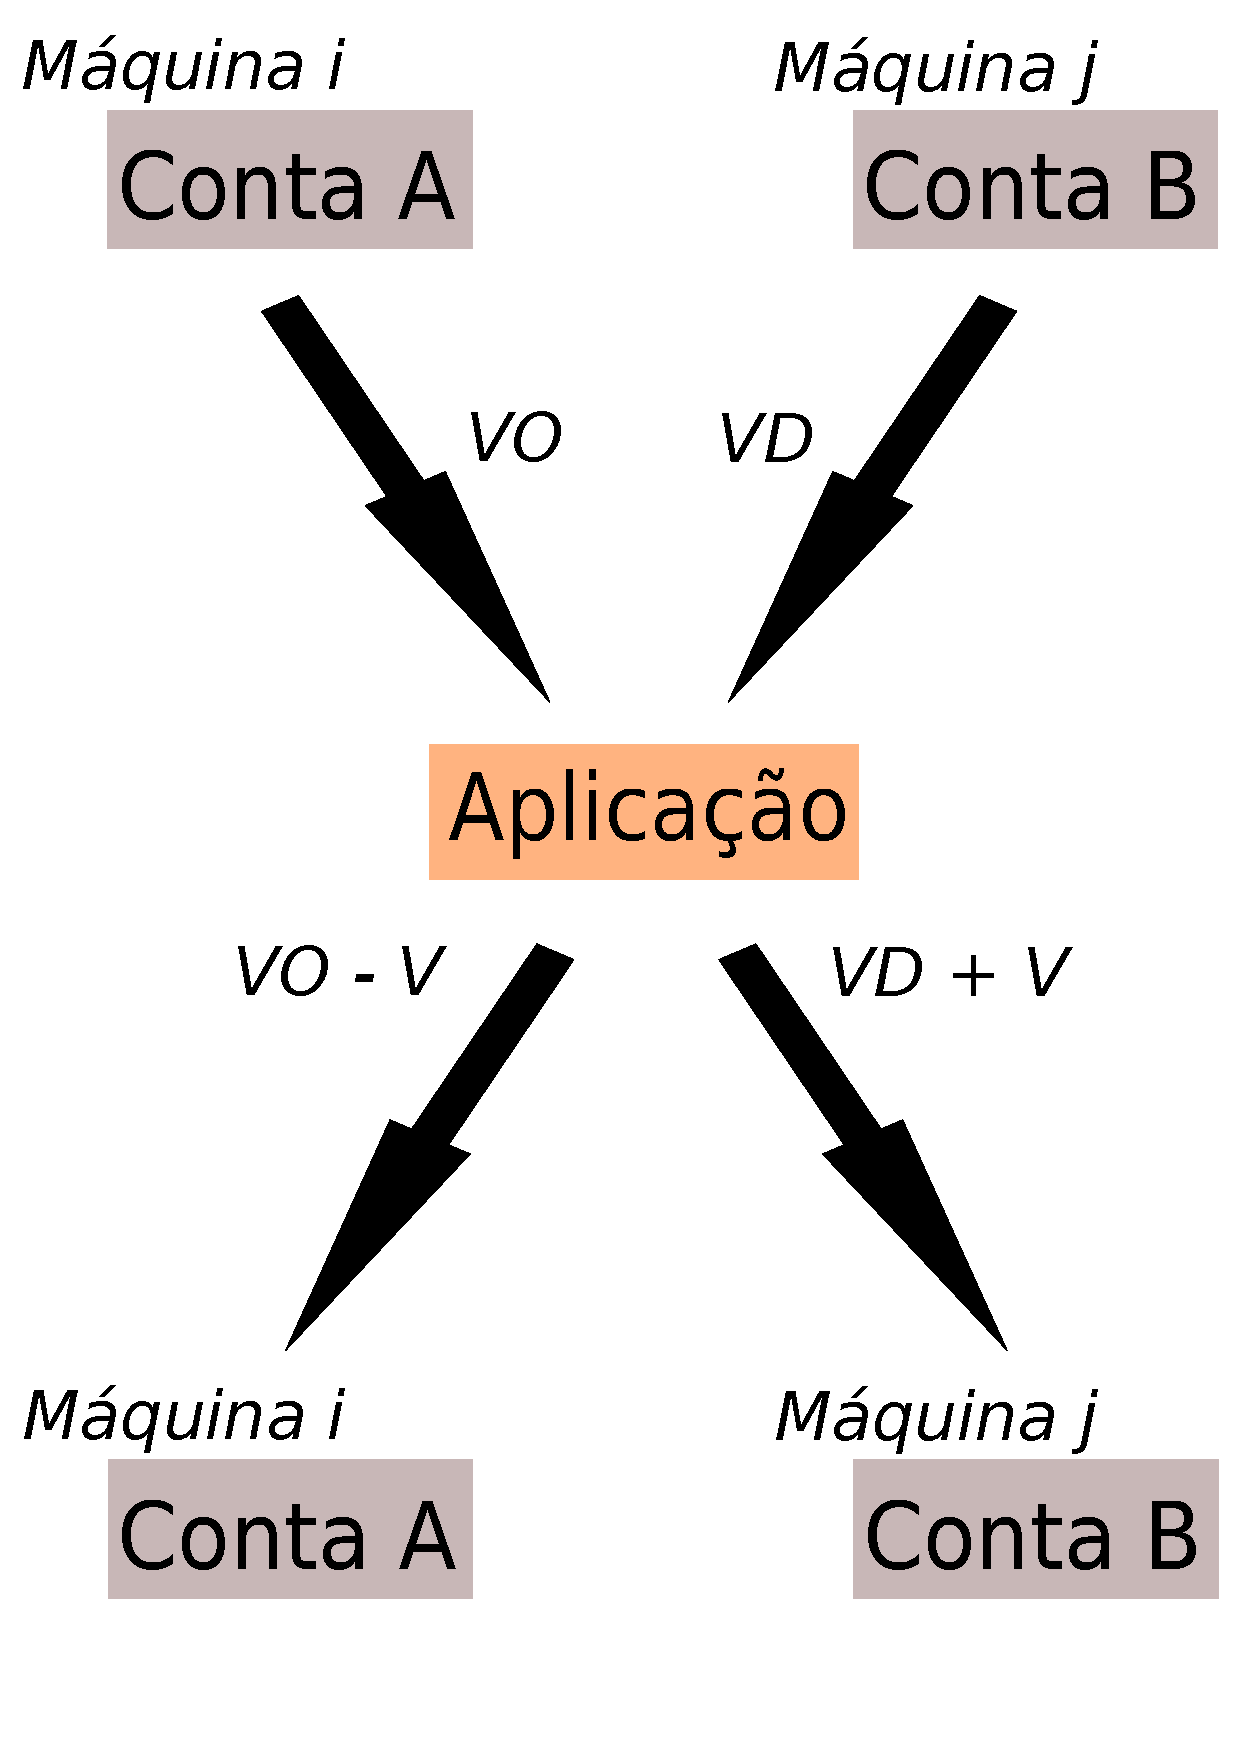
\includegraphics[width=.40\textwidth]{transacao_distribuida} 
  \caption{Esquematização de uma transação distribuída}
  \label{fig:transacao_distribuida} 
\end{figure}

A idéia desse protocolo é simples e utilizada a bastante tempo \cite{2pc}: verificar se todos os gerenciadores de recurso envolvidos em uma transação estão aptos a efetivar suas respectivas sub-transações. Se estiverem, a transação será efetivada. Se algum gerenciador não puder efetivar, por qualquer motivo, a transação será abortada. O \emph{2PC} necessita de um gerenciador que atue como o \textbf{coordenador} da transação, responsável por gerenciar a execução do protocolo e tomar a decisão sobre efetivar ou abortar a transação comunicando-se com os outros \textbf{participantes}, que executam as sub-transações associadas à transação. O coordenador pode ser um participante da transação também.

O protocolo é dividido em duas fases. Na primeira fase o coordenador solicita que os participantes enviem seus votos, indicando se estão aptos a efetivar a sub-transação executada. Os votos são coletados e o coordenador decide se a transação pode ser efetivada (caso todos os participantes tenham votado de acordo) ou se deve ser abortada (caso algum participante tenha votado para não efetivar a transação). Decidido o resultado da votação, o coordenador efetua a segunda fase, em que os participantes são notificados do resultado da votação. 

De forma mais detalhada, o \emph{2PC} pode ser descrito pelos algoritmos \ref{alg:2pc_coordenador}, \ref{alg:2pc_participante1} e  \ref{alg:2pc_participante2}. O Algoritmo \ref{alg:2pc_coordenador} descreve as ações do coordenador ao ser notificado que o protocolo deve  iniciar. Os algoritmos \ref{alg:2pc_participante1} e \ref{alg:2pc_participante2} descrevem as ações executadas pelos participantes ao receberem uma solicitação de votação (primeira fase) e o resultado da votação (segunda fase), respectivamente. 

Uma estrutura de dados essencial na execução do \emph{2PC} é o registro de operações, ou \emph{log}. Ele é responsável por registrar as decisões do coordenador e dos participantes, e é gravado localmente em cada gerenciador de recursos envolvido na transação para evitar que essas informações sejam perdidas caso ocorra alguma falha. No Algoritmo \ref{alg:2pc_coordenador} $log_c$ representa o \emph{log} do coordenador e nos algoritmos \ref{alg:2pc_participante1} e \ref{alg:2pc_participante2} $log_i$ é o \emph{log} do participante $p_i$ executando o algoritmo em questão.

A função $Adicionar$ representa a operação de adicionar um elemento ao final do \emph{log}. A função $Enviar(d, m)$ representa o envio de uma mensagem $m$ para um destinatário $d$ pela rede de comunicação, e a função $Receber(r)$ representa o recebimento de uma mensagem de um remetente $r$. Uma simulação da execução do algoritmo pode ser vista nas figuras \ref{fig:2PC_1fase} e \ref{fig:2PC_2fase}.

\begin{algorithm}
\caption{Coordenador 2PC}
\label{alg:2pc_coordenador}
\Inicio{
    $Adicionar(log_c, (PREPARAR, T))$\;
    \ParaTodo{$p_i \in Participantes$}
    {
    	$Enviar(p_i, (PREPARAR, T))$\;
    }
    $d \gets EFETIVAR$\;
    \ParaTodo{$p_i \in Participantes$}
    {    
        $v \gets Receber(p_i)$\;
        \Se{$v = ABORTAR$}
        {
            $d \gets ABORTAR$\;
        }
    }
    $Adicionar(log_c, (d, T))$\;
    \ParaTodo{$p_i \in Participantes$}
    {
    	$Enviar(p_i, (d, T))$\;
    }
}
\end{algorithm}

\begin{algorithm}
\caption{Votação 2PC - $p_i$ recebe $(PREPARAR, T)$ de $c$}
\label{alg:2pc_participante1}
\Inicio{
    $v \gets Decidir(T)$\;
    $Adicionar(log_i, (v, T))$\;
    $Enviar(c, v)$\;
}
\end{algorithm}

\begin{algorithm}
\caption{Notificação 2PC - $p_i$ recebe $(d, T)$ de $c$}
\label{alg:2pc_participante2}
\Inicio{
    \eSe{$d = EFETIVAR$}
    {
        $Efetivar(T)$\;
        $Adicionar(log_i, (EFETIVAR, T))$\;
    }
    {
    	$Abortar(T)$\;
    	$Adicionar(log_i, (ABORTAR, T))$\;
    }
}
\end{algorithm}

A premissa que norteia o protocolo é que qualquer gerenciador envolvido na transação pode decidir abortá-la de forma unilateral, ou falhar em executar uma sub-transação, exigindo assim unanimidade na decisão pela efetivação da transação. As mensagens enviadas durante a execução do protocolo indicam uma decisão do remetente, e para garantir que essa decisão sobreviva a falhas no gerenciador que enviou a mensagem, os dados do \emph{log} são gravados em um meio de armazenamento estável, como um disco rígido, antes da  mensagem ser enviada. A transação $T$ é considerada oficialmente efetivada (ou abortada) no momento que o registro de $(EFETIVAR, T)$ (ou $(ABORTAR, T)$) do \emph{log} do coordenador for escrito para a área de armazenamento estável da máquina. Falhas posteriores não podem mudar a decisão do coordenador registrada em seu \emph{log} e gravada em disco.

\begin{figure}
  \centering
  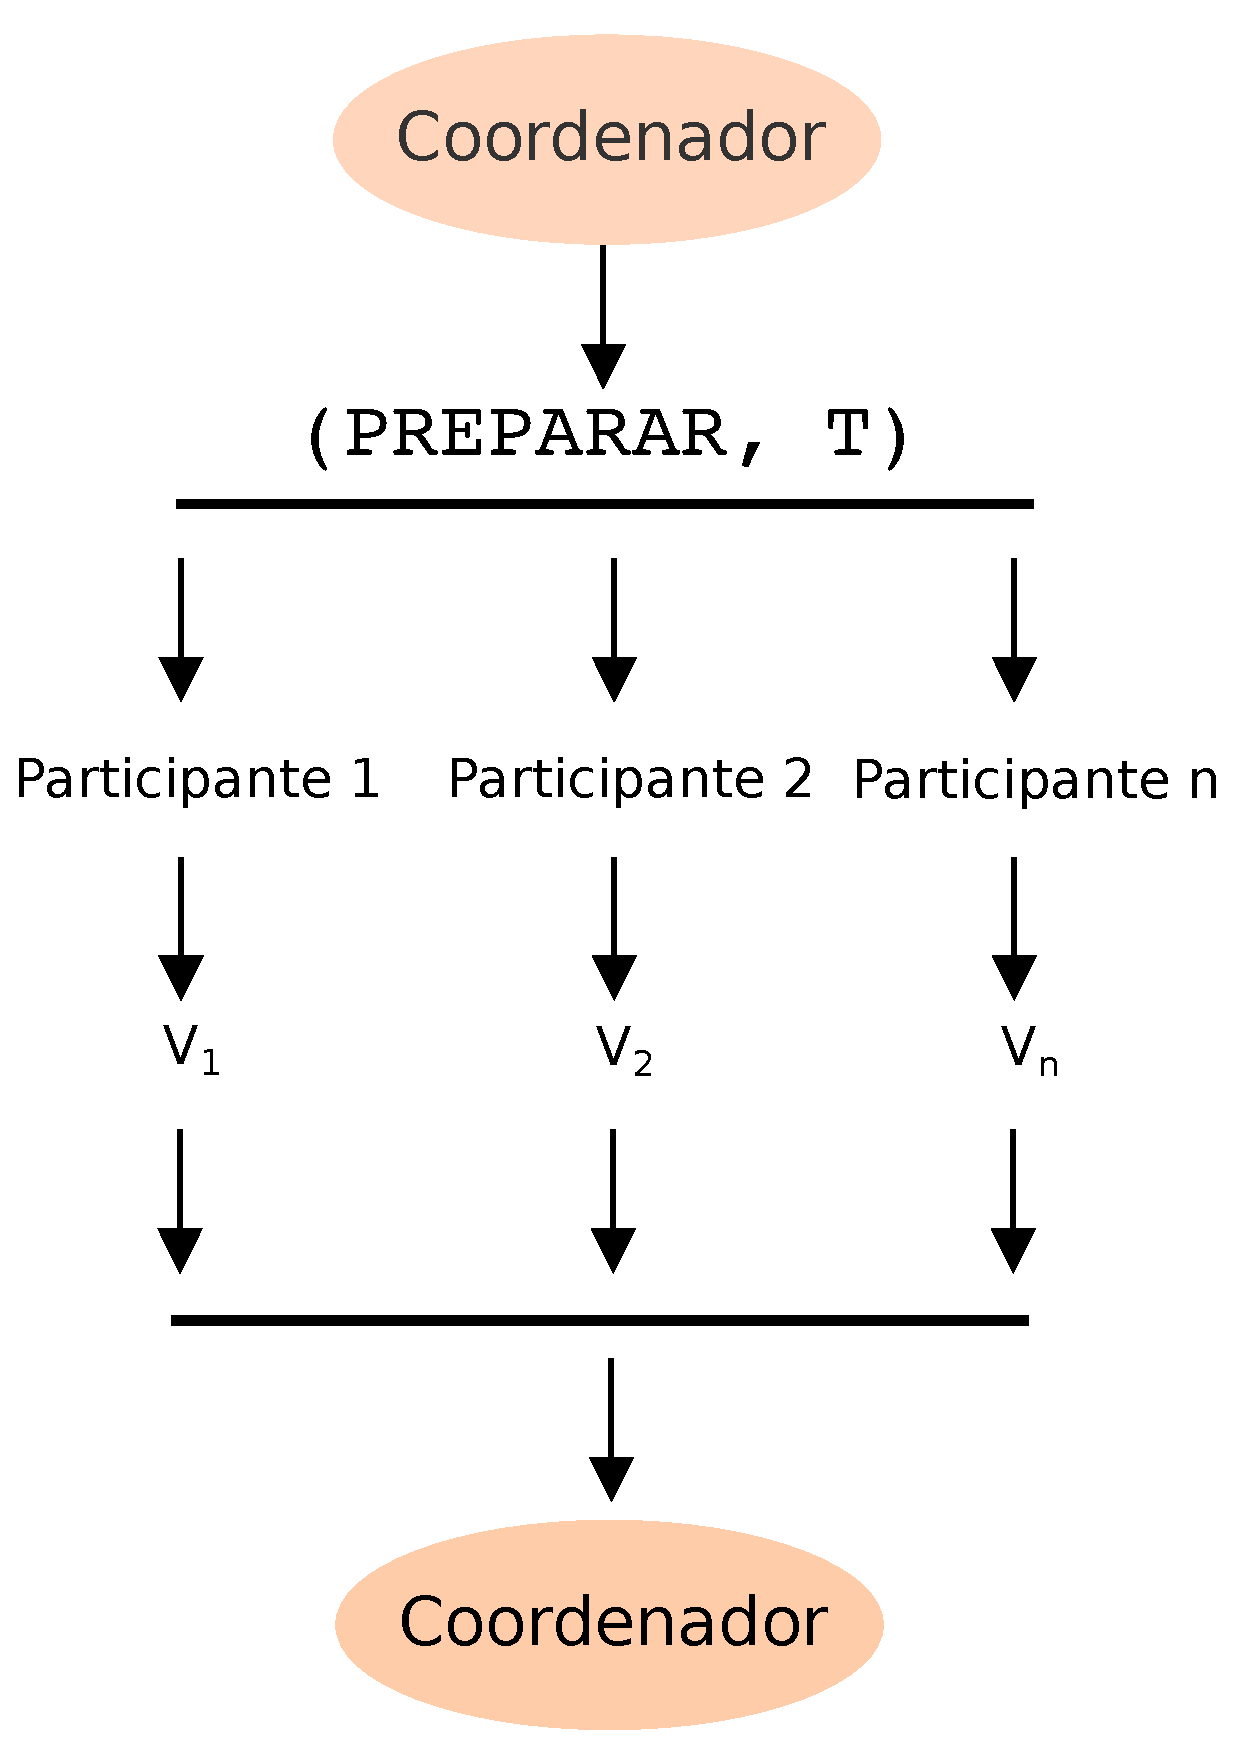
\includegraphics[width=.40\textwidth]{2PC_1fase} 
  \caption{Primeira fase 2PC - O coordenador inicia a votação e os participantes respondem com seus votos $V_i$}
  \label{fig:2PC_1fase} 
\end{figure}

\begin{figure}
  \centering
  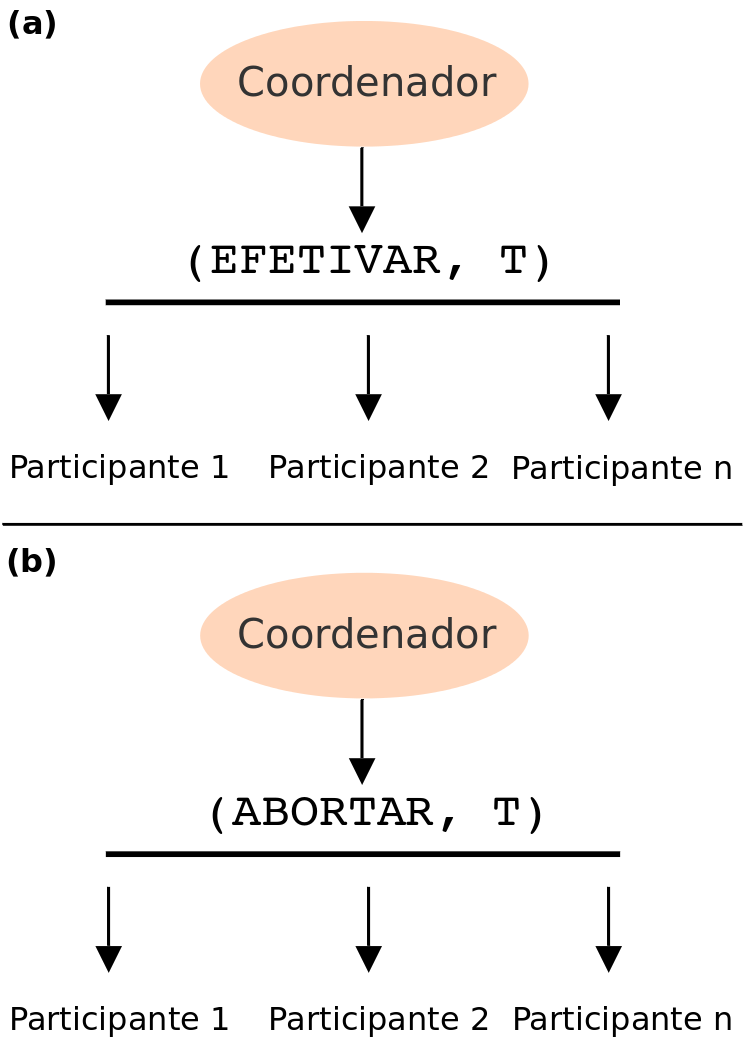
\includegraphics[width=.40\textwidth]{2PC_2fase} 
  \caption{Segunda fase 2PC- O coordenador apura os votos e notifica os participantes. Em (a) os participantes são notificados de uma efetivação. Em (b), a transação foi abortada.}
  \label{fig:2PC_2fase} 
\end{figure}

É importante notar que esse protocolo não define como as operações da transação devem ser executadas nas máquinas participantes, mas sim como a efetivação da transação deve proceder. As sub-transações ocorrem em cada participante antes que o protocolo de efetivação inicie. Portanto, a utilização desse protocolo aumenta o número de mensagens e consequentemente o tempo e o esforço necessários para que uma transação seja executada. Algumas otimizações podem ocorrer, como no caso de transações que efetuam somente operações de leitura ou de transações que envolvam dados em somente uma máquina do sistema mas, de forma geral, a execução do \emph{2PC} é custosa \cite{gray-lamport}.

\section{Minitransações}
\label{sec:minitransacoes}
Minitransação é uma primitiva que permite que as operações de uma transação sejam executadas durante o protocolo de efetivação. Esse protocolo de efetivação é uma modificação do \emph{2PC}, e oferece um mecanismo simples para ler e alterar dados de forma condicional em um ambiente distribuído garantindo atomicidade na execução das operações \cite{sinfonia}. Dessa forma, o número de mensagens e o tempo de execução da transação são reduzidos. 

Porém, o uso das minitransações impõe certas restrições em relação ao que pode ser feito, diminuindo sua aplicabilidade. Por exemplo, o condicionamento das operações de leitura e escrita é baseado somente em comparações de igualdade, e a única forma da aplicação cliente abortar a minitransação é se essa comparação falhar, como será detalhado. Com as minitransações originais não é possível efetuar a transferência entre contas distribuídas como no Algoritmo \ref{alg:transferencia_valores_transacao}, pois a comparação de maior ou igual ($>=$) não pode ser feita. A nossa infraestrutura irá permitir que essa e outras comparações sejam feitas.

Na subseção \ref{subsec:derivando-minitransacoes} é apresentado como o \emph{2PC} pode ser usado como ponto de partida para otimizações e para a obtenção do protocolo de minitransações. Na subseção \ref{subsec:estrutura-minitransacoes} definimos formalmente o conceito de minitransação.

\subsection{Otimização do \emph{2PC}}
\label{subsec:derivando-minitransacoes}
A decisão pela efetivação ou cancelamento de uma transação distribuída depende tanto de aspectos operacionais, relacionados ao ambiente de execução, quanto de aspectos semânticos, específicos do domínio da aplicação. A falha na execução de uma subtransação em alguma máquina do ambiente inviabiliza a efetivação da transação como um todo, e por isso o coordenador é forçado a cancelar a transação. Esse tipo de falha operacional não está ligada ao domínio da aplicação, mas sim ao ambiente em que essa aplicação está rodando e está, portanto, fora do controle do coordenador, que pode somente cancelar a transação e, opcionalmente, tentar executá-la novamente. Por outro lado, o aspecto semântico envolvido na decisão pela efetivação ou cancelamento da transação é específico de cada aplicação e depende, direta ou indiretamente, dos dados do sistema.

Considerando novamente o sistema bancário e a operação de transferência de uma determinada quantia entre uma conta de origem e de destino, a transferência só pode ocorrer se o saldo na conta de origem da transferência for maior ou igual à quantia a ser transferida. Essa checagem deve ser feita pela aplicação após a leitura da informação da máquina que armazena os dados da conta de origem, e a decisão pelo cancelamento ou não da transação fica subordinada à semântica dada aos dados do sistema. Isso exige que uma requisição de leitura seja feita e uma resposta seja enviada, para só então a aplicação decidir se vai efetivar e então, após a execução do restante da transação, iniciar a primeira fase do protocolo \emph{2PC} (votação).

Podemos ver que, do ponto de vista semântico, as operações que influenciam na decisão pela possível efetivação ou pelo cancelamento da transação são operações de leitura. As operações de escrita não influenciam nessa decisão, a não ser pelo ponto de vista operacional, ou seja, se ocorrer realmente um erro na operação de escrita. Assim, se tivermos uma transação cuja última ação não afete a decisão do coordenador sobre efetivar a transação, podemos embutir essa última ação na mensagem de votação da primeira fase do protocolo de efetivação.

O aspecto semântico da transação em relação aos dados pode ser tratado nos participantes também, e não somente no coordenador, caso o participante saiba como o coordenador irá utilizar o dado para fazer sua decisão sobre efetivar ou cancelar a transação. Se isso for possível, podemos então embutir também operações de leitura que influenciam a decisão do coordenador no protocolo de efetivação e fazer o participante adequar seu voto à maneira como o coordenador faria ao analisar o dado retornado.

As minitransações surgem no contexto em que todas as operações de uma sub-transação podem ser embutidas dentro do protocolo de efetivação, utilizando somente as trocas de mensagens que ocorreriam no protocolo de efetivação, após a execução dos comandos. Para que isso possa ocorrer, o protocolo \emph{2PC} precisa ser alterado.

\subsection{Definição}
\label{subsec:estrutura-minitransacoes}
Uma minitransação é composta por três conjuntos: itens de comparação, itens de leitura e itens de escrita, como pode ser visto na figura \ref{fig:estrutura_minitransacao}. Todos os itens possuem uma referência a qual dado deve ser utilizado ($ID_{A...D}$), e os itens de comparação e escrita incluem também os dados ($DADO_{1...4}$) que serão comparados com ou substituirão os dados armazenados \cite{sinfonia}. 

\begin{figure}
  \centering
  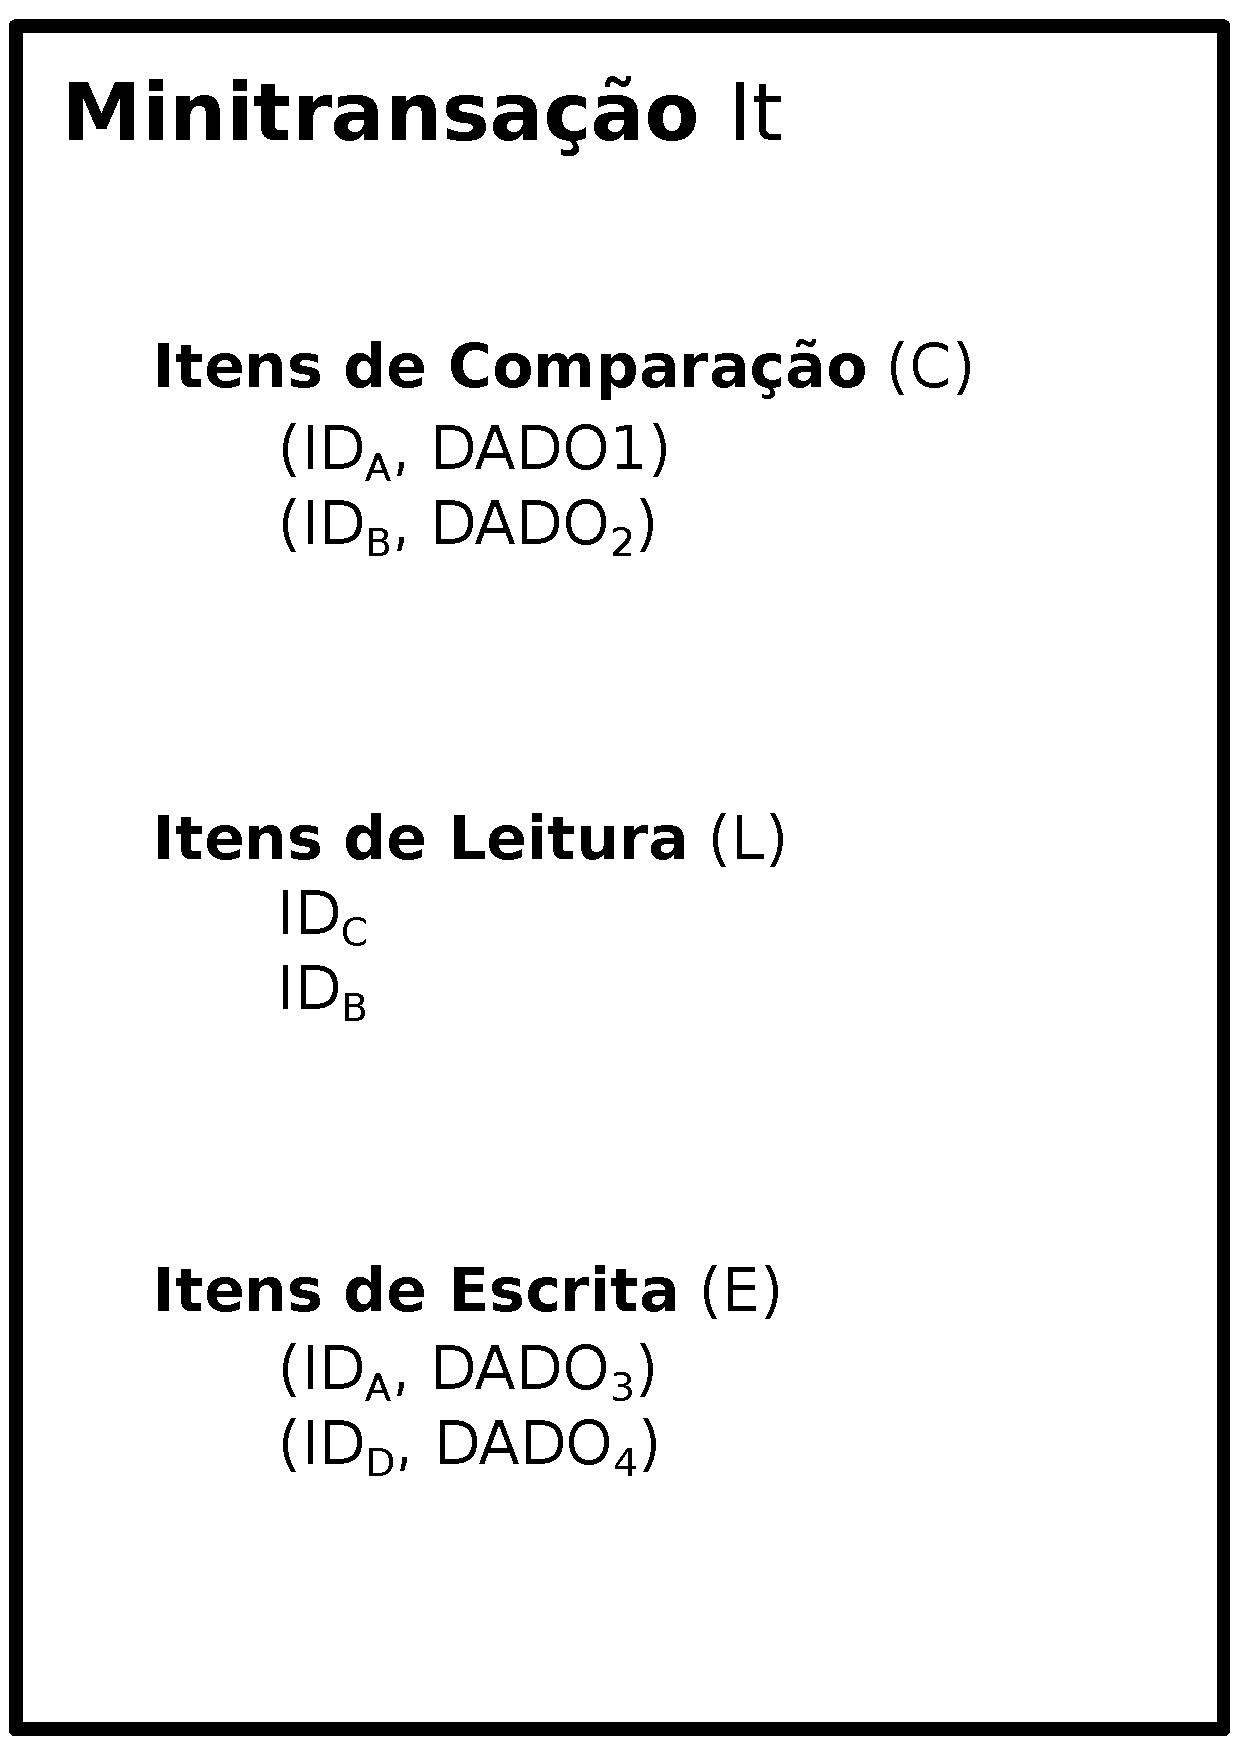
\includegraphics[width=.40\textwidth]{estrutura_minitransacao} 
  \caption{Estrutura de uma minitransação}
  \label{fig:estrutura_minitransacao} 
\end{figure}

Formalmente, uma minitransação pode ser vista como uma tupla na forma $(I, C, L, E)$. $I$ é o identificador da minitransação, gerado pelo criador da minitransação. \(C\) é o conjunto de itens de comparação, \(L\) é o conjunto de itens para leitura e \(E\) é o conjunto de itens para escrita. Os elementos de \(L\) são identificadores de dados, e o domínio de seus valores é o conjunto de identificadores armazenados na máquina participante. \(C\) e \(E\) possuem elementos que podem ser representados como tuplas no formato \((Id, Dado)\), em que \(Id\) é o identificador do dado e \(Dado\) é o valor para se comparar com o valor identificado por $Id$ ou para substituí-lo.

Sendo uma extensão do \emph{2PC}, o protocolo de minitransações possui também um coordenador responsável por iniciar e gerenciar a execução do protocolo entre os participantes da transação. O protocolo de minitransações é composto também por duas fases, mas agora a primeira fase passa a ser uma fase de execução, em que as minitransações são executadas em cada participante e seus votos são enviados para o coordenador. O coordenador coleta os votos de todos os participantes e, como no protocolo original, irá decidir por efetivar a transação somente se os votos forem unânimes. Na segunda fase os participantes são notificados da decisão do coordenador e devem atuar de acordo, efetivando as operações da minitransação ou desfazendo suas ações.

Um operador especial, $Id[X]$, representa o conjunto formado pelo elemento $Id$ de todas as tuplas no formato $(Id, Dado)$ do conjunto $X$. Esse operador permite obter o conjunto $D$ de todos os identificadores utilizados pela minitransação: $D \gets L \cup Id[C] \cup Id[E]$. Cada elemento de $D$ fica sob responsabilidade de um participante $p$ específico da minitransação, e $\forall d \in D$ o participante responsável pelo identificador $d$ é definido por $Participante(d)$, uma função que indica que $p$ é a possível localização de $d$ entre os participantes, uma vez que o identificador $d$ pode ainda não ter sido inserido em $p$.

O conjunto $Participantes$ é formado por todos os participantes da minitransação. Cada participante $P_j \in Participantes$ possui um conjunto $K_j$ de identificadores sob sua responsabilidade, e para cada participante o coordenador constrói uma nova minitransação \(M_j = (I_t, C_j, L_j, E_j)\) tal que:

\begin{itemize}
    \item $I_t \gets IdentificadorUnico(I)$
    \item $\forall i_l \in L_j, i_l \in K_j$;
    \item $\forall i_c \in Id[C_j], i_c \in K_j$; e
    \item $Id[E_j] \supseteq K_j$
\end{itemize}

O identificador $I_t$ é unicamente definido e associado ao identificador $I$ por meio da função $IdentificadorUnico$. Como o identificador $I$ é fornecido pela aplicação cliente, nada garante que ele seja único, e por isso utilizamos $IdentificadorUnico$ para criar um novo identificador globalmente único associado à $I$. Os identificadores de $E_j$ são tratados como um superconjunto de $K_j$ pois a operação de escrita pode inserir novos dados no sistema, e não somente alterar dados que já existem.

Cada $M_j$ é enviada ao respectivo $P_j$ pelo coordenador, que irá esperar pela execução e resposta de cada participante. Ao receber uma minitransação, cada participante irá tentar ler os dados identificados por $Id[C_j]$ e compará-los (comparação de igualdade) com os respectivos $Dado[C_j]$. Caso a comparação não seja bem sucedida, esse participante nem tentará ler ou modificar os dados em $L_j$ e $E_j$, e responderá para o coordenador com um voto $ABORTAR$. A Figura \ref{fig:minitransacao_1fase} ilustra essa primeira fase, que combina a primeira fase do \emph{2PC} com a execução das operações da transação.

\begin{figure}
  \centering
  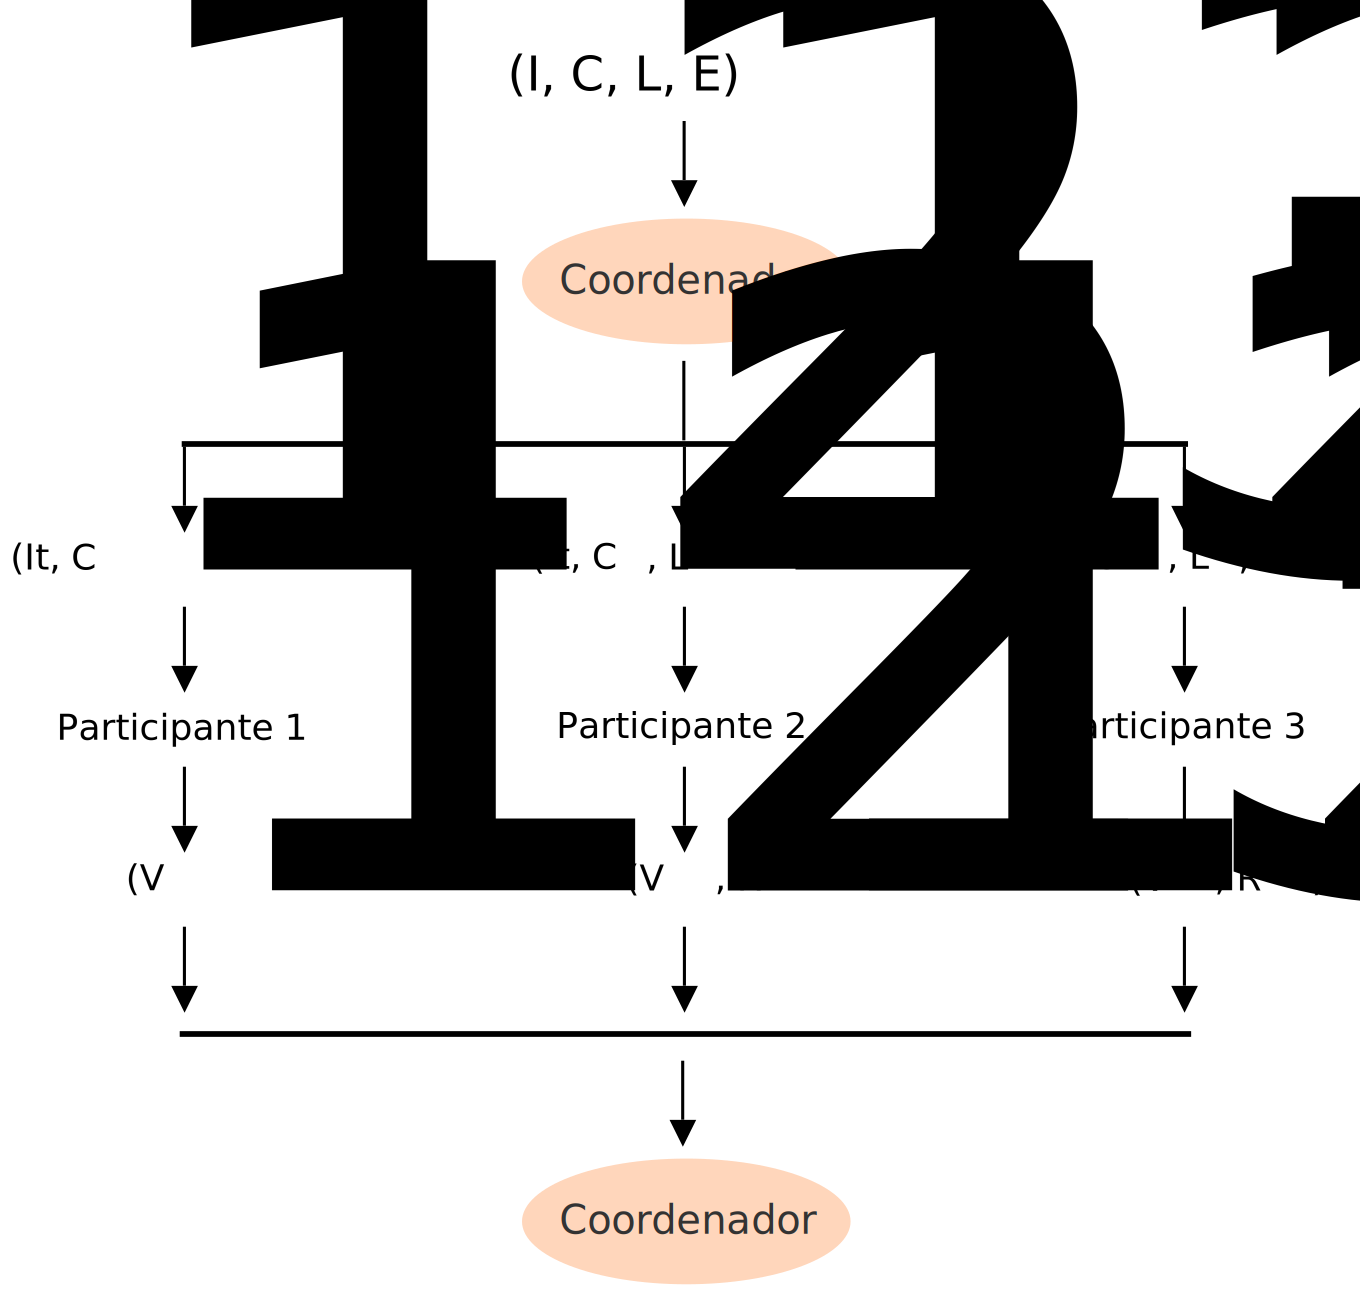
\includegraphics[width=.65\textwidth]{minitransacao_1fase} 
  \caption{Fase de execução de uma minitransação}
  \label{fig:minitransacao_1fase} 
\end{figure}

Se a comparação for bem sucedida para todos os elementos de $Id[C_j]$, então o participante irá ler os dados identificados por $L_J$ e agrupá-los no conjunto de resposta $R_j$. Os dados $Dado[E_j]$ identificados por $Id[E_j]$ serão inseridos no conjunto de dados ou irão alterar algum dado já existente. Na verdade, a operação de inserir ou alterar um dado é registrada no \emph{log} do participante. O participante envia então um voto $EFETIVAR$ para o coordenador, junto com o conjunto $R_j$. 

Ao coletar todas as respostas, o coordenador irá apurar os votos de cada participante. Para cada resposta $EFETIVAR$ o coordenador agrega os respectivos $R_j$ em um conjunto de respostas $R$. Se uma das respostas for $ABORTAR$, a transação precisa ser abortada, notificando os participantes do cancelamento, e a aplicação cliente precisa ser notificada desse erro, como podemos ver na Figura \ref{fig:minitransacao_2fase} \textbf{b}. Se não houve nenhum voto $ABORTAR$, o coordenador decide então por efetivar a transação, enviando o conjunto $R$ para a aplicação cliente e notificando os participantes da efetivação, como ilustrado na Figura \ref{fig:minitransacao_2fase} \textbf{a}.

\begin{figure}
  \centering
  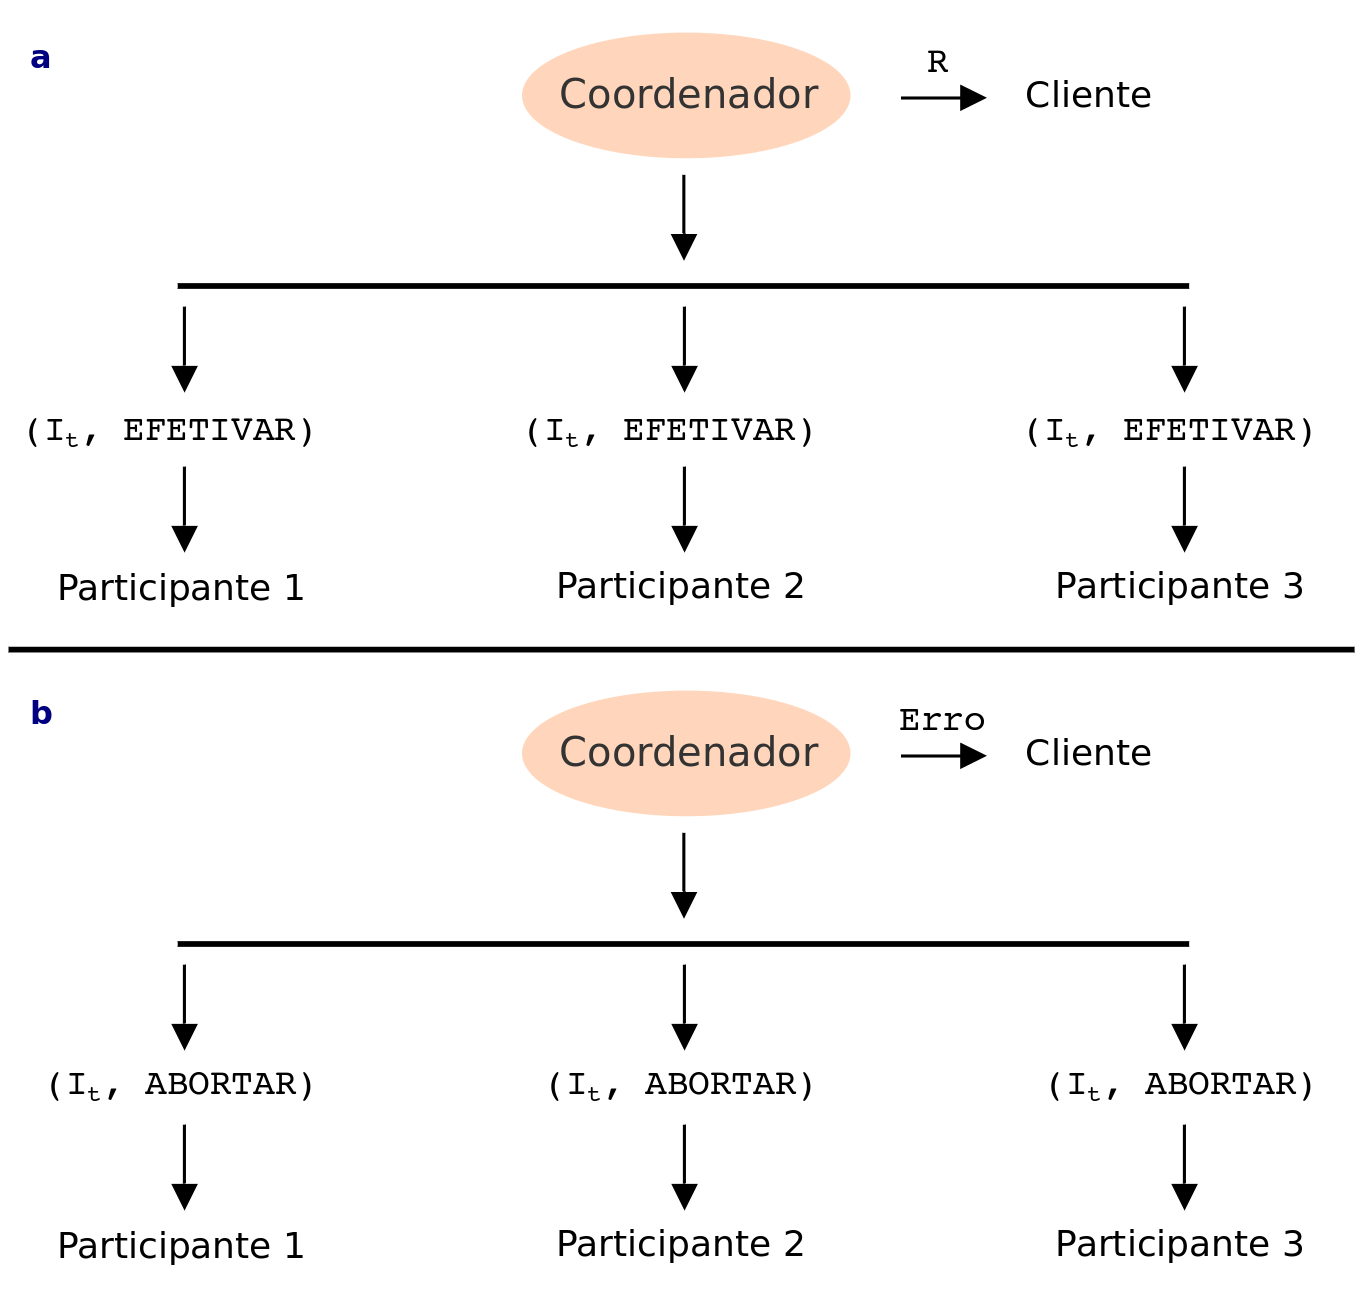
\includegraphics[width=.65\textwidth]{minitransacao_2fase} 
  \caption{Fase de notificação de uma minitransação}
  \label{fig:minitransacao_2fase} 
\end{figure}

Quando os participantes são notificados do cancelamento da minitransação, as operações de escrita da minitransação presentes no \emph{log} do participante não serão efetuadas, deixando os dados inalterados, e será registrado no \emph{log} que a minitransação foi abortada. Se a notificação for de efetivação, as operações de escrita do \emph{log} serão efetuadas, alterando dados existentes ou inserindo novos dados no participante, e será registrado no \emph{log} que a minitransação foi efetivada. O \emph{log} será gravado em disco e a minitransação será considerada oficialmente efetivada ou abortada no momento que esse registro do \emph{log} estiver gravado em disco.

\chapter{A infraestrutura}
\label{chap:implementacao}
Na seção \ref{sec:infinispan} apresenta o Infinispan, detalhando os pontos importantes de sua arquitetura e parte central de sua implementação. 

A seção \ref{sec:mt_infinispan} descreve como as minitransações se encaixam na estrutura de transações do Infinispan e as alterações que foram necessárias nessa estrutura para disponibilizar as minitransações.

\section{Infinispan}
\label{sec:infinispan}
O Infinispan foi escolhido como base para o desenvolvimento de nossa infraestrutura por ser uma plataforma e repositório de dados distribuído. Além disso, ele é um sistema de código aberto, escrito em \emph{Java} \cite{java}, projetado para expor uma estrutura de dados altamente concorrente e para obter o melhor desempenho das modernas arquiteturas de múltiplos processadores e múltiplos núcleos, ao mesmo tempo em que oferece funcionalidades de \emph{cache} distribuído.

Na seção \ref{sec:arquitetura_infinispan} descrevemos a arquitetura do Infinispan, e os principais conceitos sobre os quais essa arquitetura se baseia. A seção \ref{sec:implementacao_infinispan} detalha o núcleo de código que habilita os pontos centrais dessa arquitetura.

\subsection{Arquitetura}
\label{sec:arquitetura_infinispan}
As máquinas rodando Infinispan podem formar um ou mais agrupamentos (\emph{cluster}), caso sejam configuradas de tal forma. Esses agrupamentos permitem que os dados sejam espalhados por diferentes máquinas, permitindo assim uma melhor distribuição de carga entre as máquinas e aumento na disponibilidade dos dados.

O componente principal do Infinispan é a interface \emph{org.infinispan.Cache}, uma extensão da interface \emph{java.util.Map} da biblioteca padrão de coleções do \emph{Java}. O acesso aos dados segue então a mesma abordagem, armazenando entradas, em que um valor é associado a uma chave arbitrária definida pela aplicação. \emph{Cache} permite abstrair os diversos modos de execução em que o Infinispan pode rodar, oferecendo uma interface simples e de ampla utilização para acessar os dados.

Os quatro modos de execução oferecidos pelo Infinispan são:

\begin{description}
	\item[Local] Todas as entradas são armazenadas na máquina local, mesmo que um agrupamento tenha sido formado.
	\item[Replicado] Todas as entradas são copiadas para todas as outras máquinas do agrupamento.
	\item[Distribuído] Cada entrada é replicada para um subconjunto das máquinas do agrupamento.
\end{description}

No modo \textbf{Local} todas as entradas ficam armazenadas na mesma máquina em que o cache está configurado, não permitindo que aplicações compartilhem os dados. O modo \textbf{Replicado} garante alta disponibilidade dos dados, uma vez que cada entrada está copiada em todas as máquinas do agrupamento. Assim, um dado só ficará indisponível no caso em que todas as máquinas do agrupamento em que ele esteja armazenado fiquem indisponíveis. No modo \textbf{Distribuído} o Infinispan armazena uma determinada entrada em um subconjunto do agrupamento. Dessa forma, se esse subconjunto de máquinas ficar indisponível, essa determinada entrada ficará indisponível também. 

O modo \textbf{Distribuído} permite um certo grau de disponibilidade ao mesmo tempo em que oferece um espaço de armazenamento expandido compartilhado entre o agrupamento. Esse grau de disponibilidade é controlado pelo tamanho do subconjunto em que uma entrada será replicada, podendo variar de 1 (não havendo nenhuma replicação, cada entrada é armazenada em somente uma máquina) até o total de máquinas no agrupamento (o que fará esse modo idêntico ao \textbf{Replicado}). O grau de expansão do espaço de armazenamento é inversamente proporcional à disponibilidade, ou seja, quanto maior a disponibilidade, menor a expansão, pois menos espaço ficará disponível devido ao maior número de cópias de uma entrada.

O Infinispan oferece também duas modalidades de acesso:

\begin{description}
	\item[Embarcado]
	\item[Cliente-Servidor] 
\end{description}

Na modalidade de acesso \textbf{embarcado}, o espaço de armazenamento do Infinispan compartilha a mesma máquina virtual \emph{Java} (e portanto, a mesma memória) que a aplicação. No modo \textbf{cliente-servidor}, uma máquina virtual fica dedicada ao espaço de armazenamento do Infinispan, e a aplicação pode acessar esse espaço por meio de alguns protocolos disponíveis: HTTP, Memcached ou HotRod \cite{infinispan}.

As máquinas que compõem o agrupamento (os nós) formam uma rede \textbf{P2P} (\emph{Peer-to-Peer} ou ponto-a-ponto \cite{p2p}). Em uma rede P2P, cada participante (cada nó rodando o Infinispan) compartilha uma parcela de seus próprios recursos (processador, memória, 
etc...) para oferecer um serviço em conjunto com todos os outros participantes (nesse caso, oferecer uma abstração de cache distribuído).
O ponto central dessa rede P2P é que não há distinção entre os nós. Cada nó pode atuar tanto como um provedor quanto como um solicitante de recursos. Qualquer nó pode receber uma solicitação para armazenar ou recuperar um dado associado a qualquer chave, e essa solicitação será atendida de forma transparente por meio da cooperação entre os nós que compõem a rede.

O que permite essa transparência no acesso e independência de localização é uma abstração conhecida como \textbf{DHT} (\emph{distributed hash table}, ou tabela de espalhamento distribuída \cite{dht}). Em uma DHT, existe um conjunto finito de localizadores, e a cada nó que compõe a rede é atribuída a tutela sobre um determinado subconjunto desses localizadores. A DHT permite então encontrar ou armazenar um par de chave e valor por meio do mapeamento da chave para um determinado localizador, que por sua vez está sob a tutela de um nó da rede.

A associação entre localizadores e um nó é feito por uma função de espalhamento consistente (\emph{consistent hashing} \cite{consistent_hashing}), que é um tipo especial de função de espalhamento (\emph{hash function} \cite{taocp_3}). Como toda função de espalhamento, ela mapeia um conjunto de valores para um índice em um espaço de endereçamento (um localizador) de uma forma que a cada localizador desse espaço sejam mapeados subconjuntos com aproximadamente o mesmo tamanho. A propriedade essencial da função de espalhamento consistente que a torna de grande utilidade em um ambiente distribuído é que, ao contrário dos outros tipos de funções de espalhamento, um pequena alteração no espaço de endereçamento resulta em um número pequeno e limitado de remapeamento, mantendo a maioria dos valores mapeados para os mesmos localizadores.

\subsection{Implementação do Infinispan}
\label{sec:implementacao_infinispan}
Infinispan é implementado integralmente na plataforma java, versão padrão (\emph{SE} ou \emph{Standard Edition}). Dessa forma é possível executar o Infinispan em qualquer sistema operacional e plataforma de máquina que ofereça suporte à essa versão do java. Seu código é aberto e público, o que permitiu sua utilização como base para o desenvolvimento de nossa infraestrutura.

A natureza distribuída do Infinispan exige que os nós se comuniquem por meio da rede, e o Infinispan utiliza o JGroups \cite{jgroups} para isso. JGroups oferece uma camada de abstração sobre a rede permitindo um mecanismo de troca de mensagens confiável entre um ou mais nós de uma só vez, que o Infinispan utiliza para a formação dos agrupamentos e comunicação entre os nós.

A interface Cache é uma extensão da interface \emph{java.util.concurrent.ConcurrentMap}, que por sua vez extende \emph{java.util.Map}. \emph{Map} permite armazenar e recuperar entradas compostas por uma chave e um valor, além de possuir alguns outros comandos úteis, como para verificar se uma determinada chave foi armazenada, ou consultar o número de entradas armazenadas. A interface \emph{ConcurrentMap} introduz alguns comandos úteis para a utilização de um mapa em um ambiente de código concorrente, como um comando para armazenar uma entrada somente se a chave associada não tiver sido mapeada (\emph{putIfAbsent}) ou para trocar o valor de uma entrada baseado em um valor já existente (\emph{replace}). A interface Cache acrescenta as funcionalidades para a representação de um cache distribuído e outras funcionalidades específicas para a manutenção e utilização dos agrupamentos formados no Infinispan.

Infinispan começou a ser desenvolvido em paralelo à especificação da JSR-107 \cite{jsr107}, uma padronização ao acesso de mecanismos de cache em java. Essa especificação define uma interface \emph{javax.cache.Cache} que é muito parecida com a interface Cache do infinispan, mas que não disponibiliza acesso a todos os recursos presentes no infinispan. Assim, para poder adequar e permitir que o infinispan possa ser usado por aplicações acessando caches por meio da JSR-107, foi criado o AdvancedCache, uma interface que estende Cache e permite acessar detalhes específicos do infinispan como adicionar e remover interceptadores, gerenciadores de travas e etc. A interface Cache é compatível com a interface de mesmo nome da JSR-107, enquanto que AdvancedCache acrescenta o que é específico do infinispan.

\emph{CacheImpl} é a classe que implementa AdvancedCache (e portanto, Cache). Ela converte as chamadas das funções da interface em comandos representando as ações a serem executadas, contendo referências e informações necessárias para essa execução. Esses comandos são executados por diferentes tipos de processadores de comandos, cada um responsável por diferentes aspectos que um comando apresenta (como distribuição na rede ou persistência de dados em disco). Os processadores são dispostos em uma sequência configurada, e a execução do comando é composta então pela atuação de cada um desses processadores, um após o outro, seguindo a sequência estabelecida. Esse esquema de execução é baseado em alguns padrões (\emph{design patterns}) bem estabelecidos e de ampla utilização, como \emph{Command}, \emph{Visitor}, \emph{Chain of Responsibility} e \emph{Interceptor} (\cite{design_patterns}, \cite{posa}).

Por exemplo, a operação \emph{Cache.get(Object k)}, que permite recuperar a entrada associada à chave \emph{k}, é transformada no comando \emph{GetKeyValueCommand}. De acordo com a configuração e detalhes específicos de cada cache, a sequência de processadores pode ser ligeiramente diferente, mas os tipos mais representativos de processadores são:

\begin{description} 
	\item[DistributionInterceptor] - Provê funcionalidades básicas para que o cache opere de forma distribuída. Processadores mais específicos como \textbf{TxDistributionInterceptor} e \textbf{NonTxDistributionInterceptor} estendem a classe base e são usados de acordo com a configuração para obter melhor desempenho.
	\item[LockingInterceptor] - Gerencia a aquisição e liberação de travas em chaves ou grupos de chaves. Conforme a configuração, são utilizadas classes mais especializadas como \textbf{OptimisticLockingInterceptor} ou \textbf{PessimisticLockingInterceptor}.
	\item[TxInterceptor] - Responsável por tratar de aspectos transacionais, como registrar o cache como um participante em uma transação distribuída.
	\item[CallInterceptor] - Sempre posicionado como o último processador na sequência, é responsável por invocar a operação específica de cada comando.
\end{description}

Um componente muito importante na execução de um comando é InvocationContext, a interface principal da hierarquia ilustrada na figura \ref{fig:invocation_context}, e a escolha de uma ou outra implementação é determinada em tempo de execução de acordo com a configuração. InvocationContext contém informações como o endereço de origem da execução e as chaves sobre as quais a execução obteve travas. AbstractInvocationContext provê a base necessária para a implementação dos contextos, implementando os métodos definidos em InvocationContext de maneira direta. NonTxInvocationContext é utilizado quando o cache não está configurado para utilizar transações, e SingleKeyNonTxInvocationContext é uma otimização para quando a operação envolve somente uma chave. TxInvocationContext permite acessar a transação associada à execução pode ser de dois tipos: LocalTxInvocationContext ou RemoteTxInvocationContext. A implementação Local é utilizada para operações transacionais que foram iniciadas no mesmo nó que estiver executando a operação, e Remote é utilizada quando a operação tiver sido iniciada em um outro nó. 

\begin{figure}
  \centering
  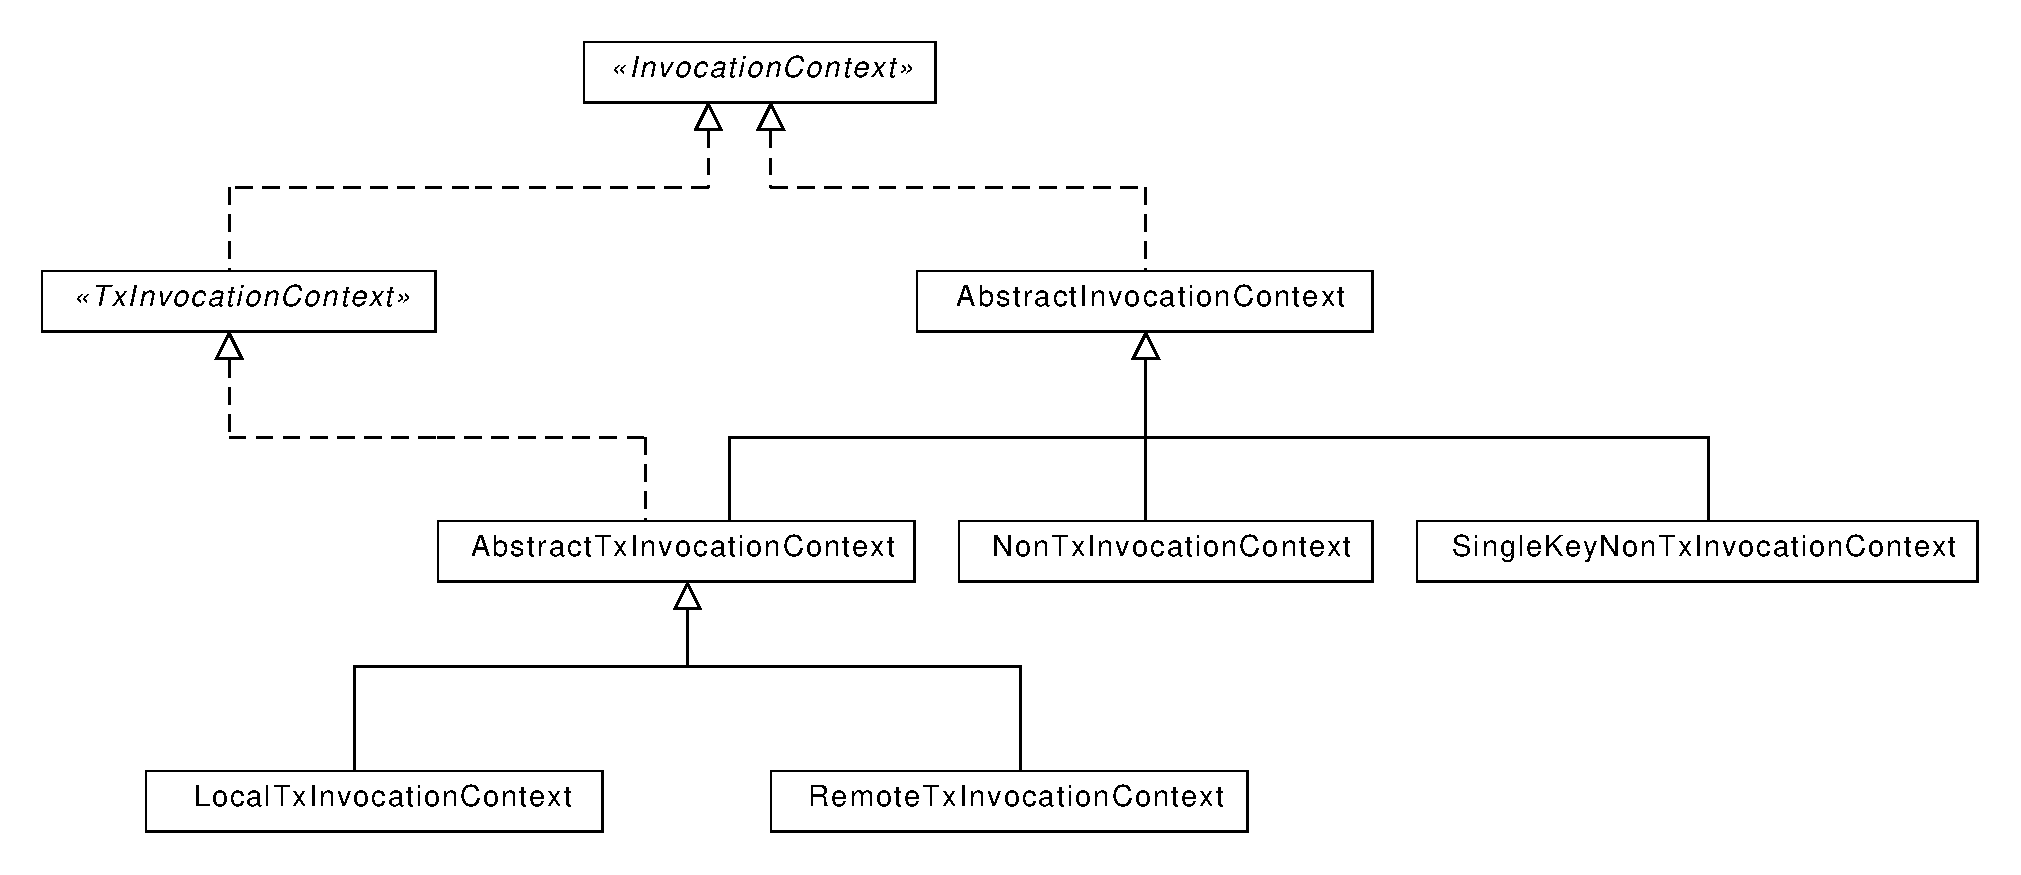
\includegraphics[width=\textwidth]{invocation_context} 
  \caption{Hierarquia de InvocationContext}
  \label{fig:invocation_context} 
\end{figure}

\section{Minitransações no Infinispan}
\label{sec:mt_infinispan}
O subsistema de transações do Infinispan permite agrupar operações em unidades lógicas de execução, oferecendo uma opção transacional para quem utiliza o cache. A seção \ref{sec:tx_infinispan} detalha o subsistema que gerencia e executa transações dentro do Infinispan. A seção seguinte, \ref{sec:suporte_mt_infinispan}, apresenta as modificações necessárias nesse subsistema para que o Infinispan permita a execução de minitransações.

\subsection{O subsistema de transações do Infinispan}
\label{sec:tx_infinispan}
O Infinispan pode ser configurado para agrupar ou não as operações em transações. Quando configurado para não agrupar, cada operação efetuada no cache é considerada isolada, sem relação com as outras operações. Nessa configuração, cada operação pertence a uma transação distinta, que é iniciada antes da operação ser executada e finalizada após o término da execução da operação.

Quando configurado para agrupar as operações, o Infinispan permite que o usuário defina as operações que formam uma transação, explicitamente iniciando e finalizando uma transação de modo a englobar as operações que precisam ser executadas como uma única operação lógica.

A abstração central do subsistema de transações é CacheTransaction, uma \emph{interface Java} \cite{java} que define os detalhes de uma transação no Infinispan. CacheTransaction é o topo de uma complexa estrutura projetada para atender a diferentes demandas transacionais e permitir a integração com \emph{JTA} (\emph{Java Transaction API} \cite{jta}) e \emph{X/Open XA} (\emph{Extended Architecture} \cite{xa}). Um resumo dessa estrutura é apresentado na figura \ref{fig:subsistema_transacoes}.

\begin{figure}
  \centering
  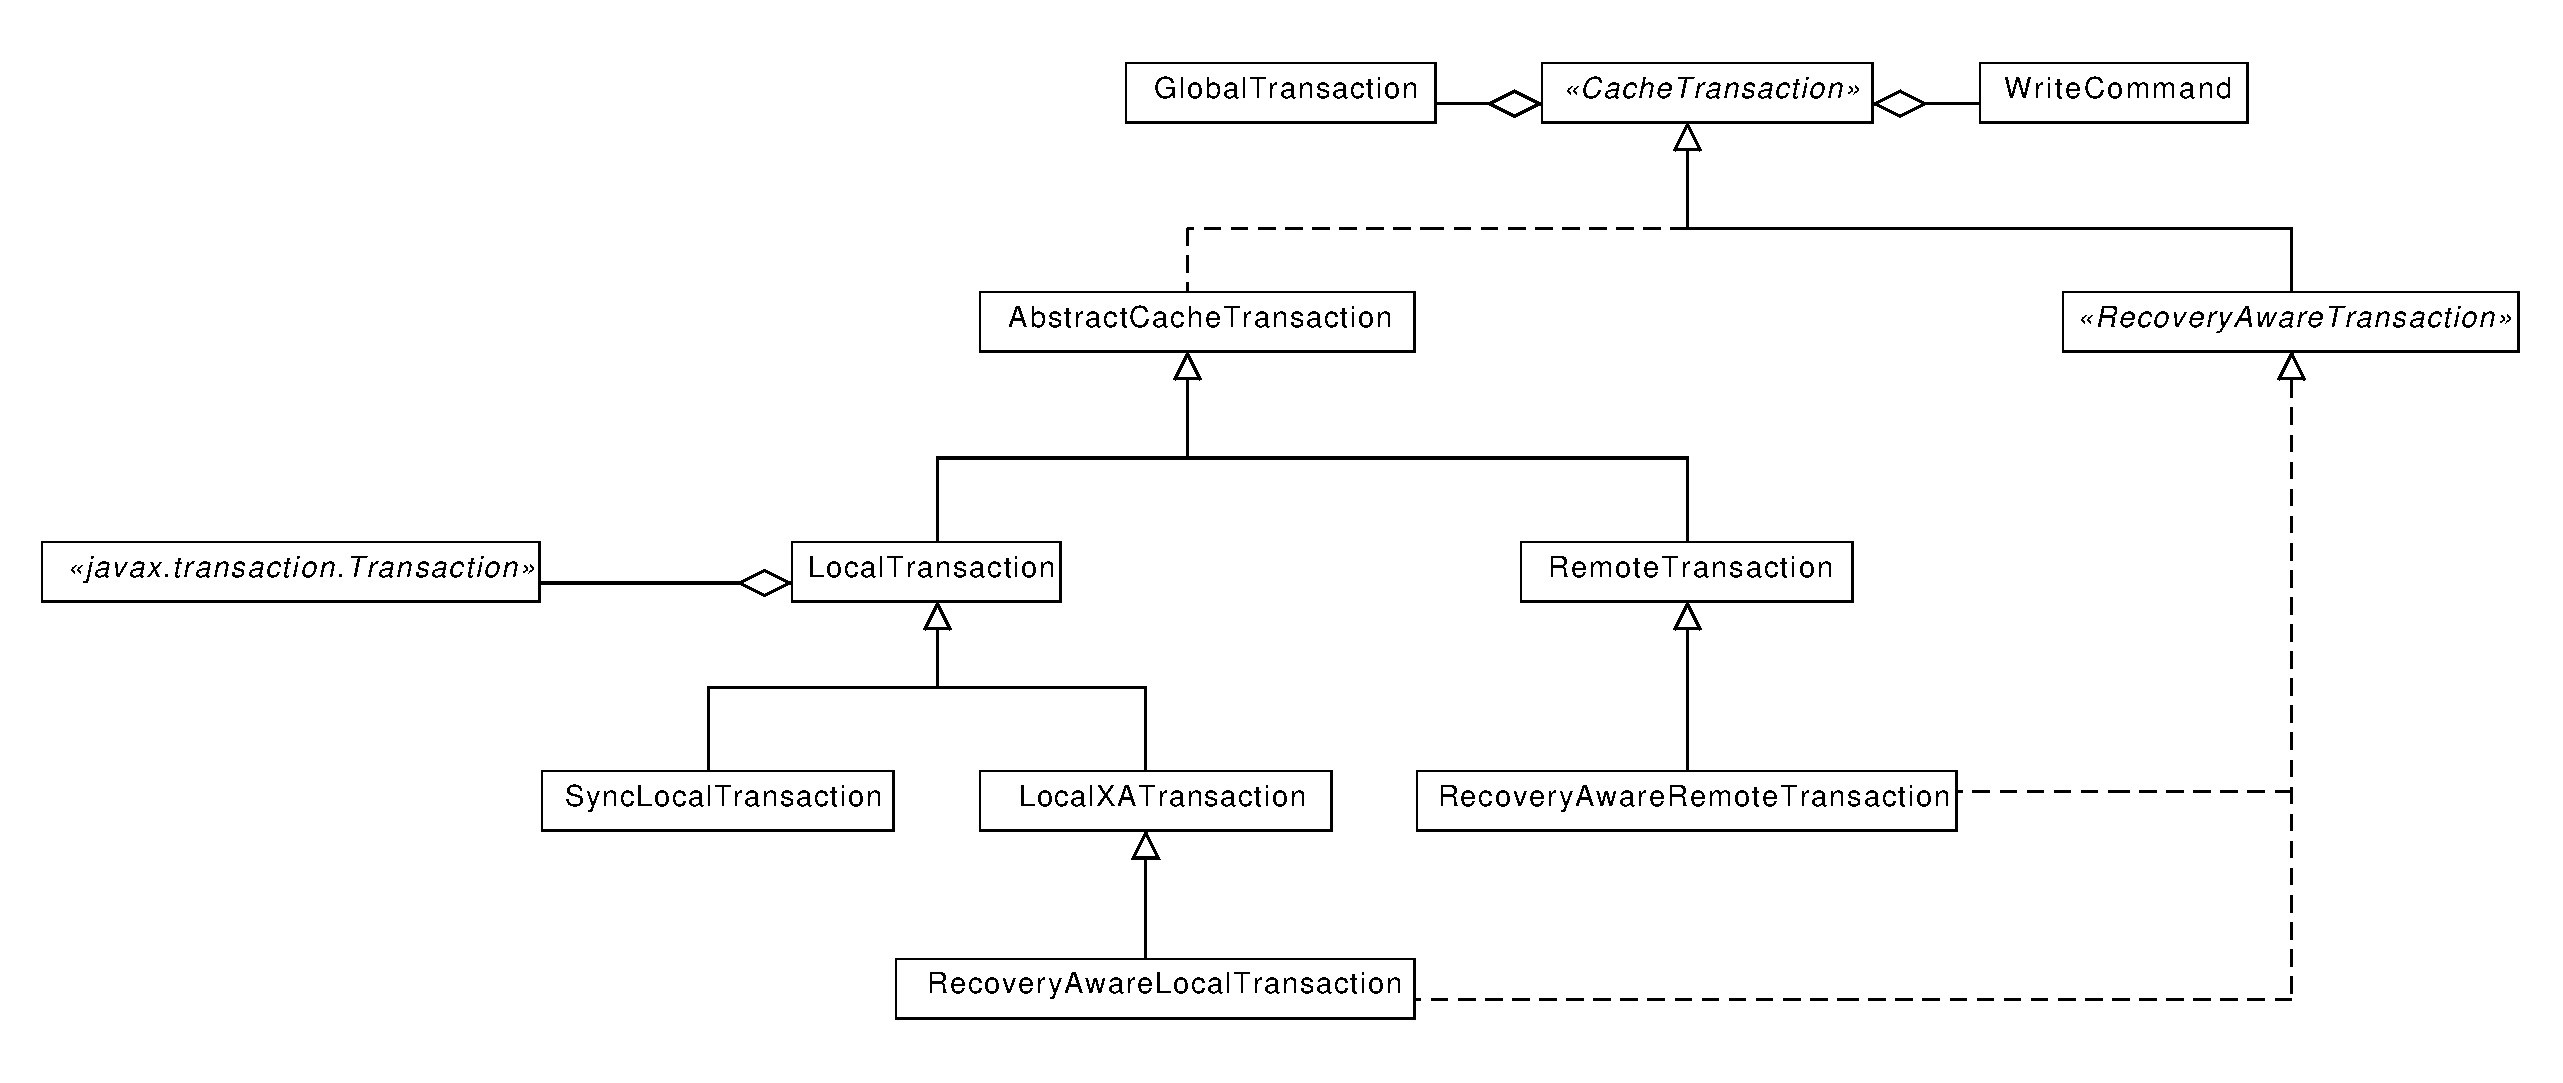
\includegraphics[width=\textwidth]{subsistema_transacoes} 
  \caption{Resumo do subsistema de transações}
  \label{fig:subsistema_transacoes} 
\end{figure}

LocalTransaction é utilizada na execução de transações iniciadas localmente e RemoteTransaction representa uma transação em execução em um nó A que foi iniciada em um outro nó B do agrupamento e que altera informações sob a responsabilidade de A. A classe LocalTransaction referencia uma Transaction do JTA. SyncLocalTransaction é utilizada por SynchronizationAdapter, que implementa a interface Synchronization definida pela JTA. LocalXATransaction é utilizada pelo TransactionXAAdapter, que implementa XAResource para integração com gerenciadores compatíveis com XOpen/XA. Tanto SynchronizationAdapter quando TransactionXAAdapter mapeiam chamadas do JTA e XOpen/XA, respectivamente, para operações de TransactionCoordinator, que centraliza a lógica para o controle de estado e execução das transações. O relacionamento entre essas classes pode ser visto na figura \ref{fig:transaction_coordinator}

\begin{figure}
  \centering
  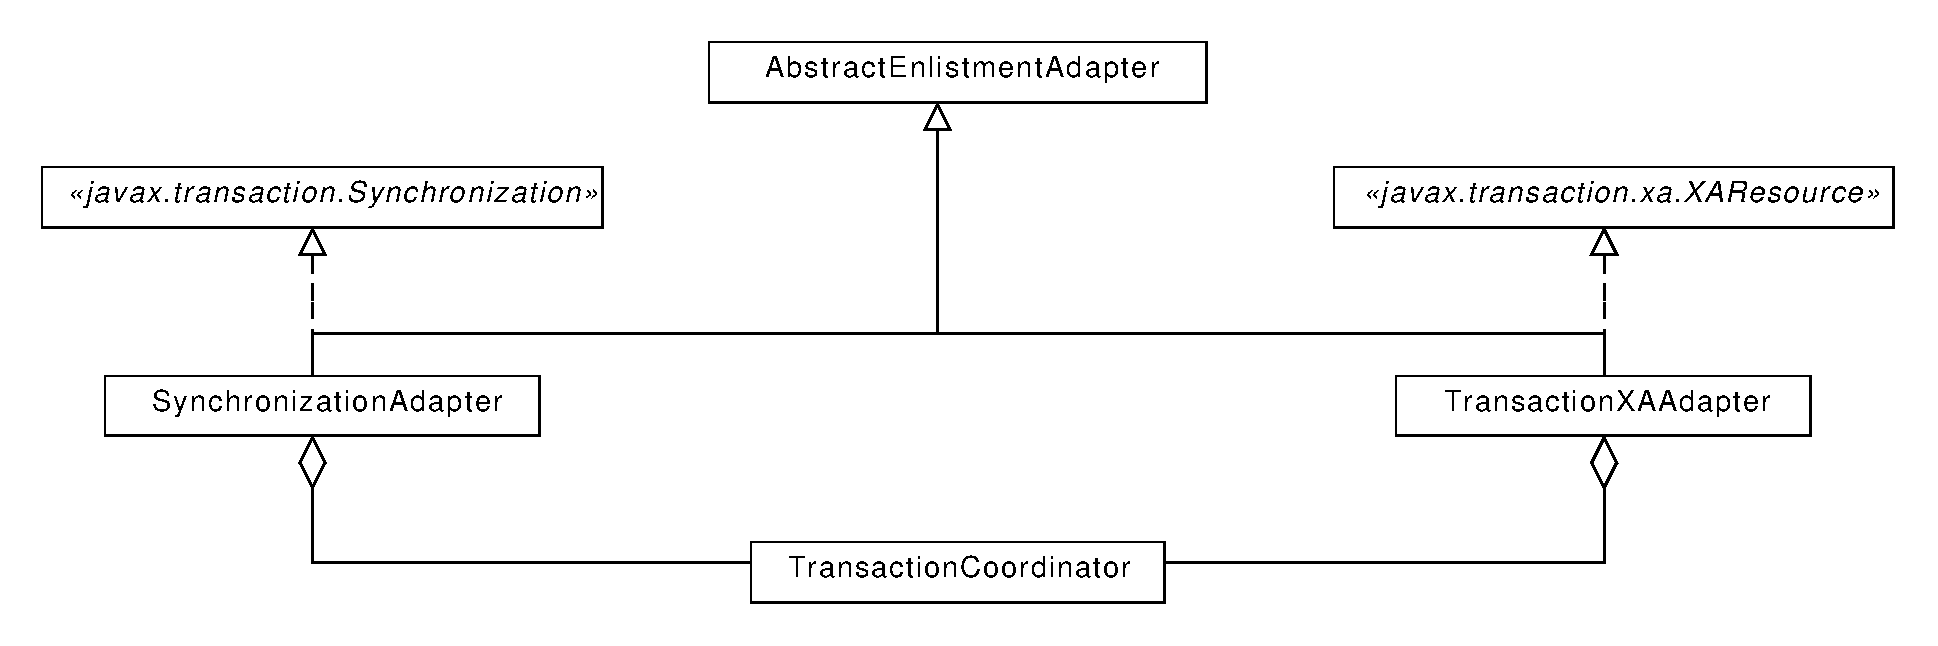
\includegraphics[width=\textwidth]{transaction_coordinator} 
  \caption{TransactionCoordinator e seus adaptadores}
  \label{fig:transaction_coordinator} 
\end{figure}

GlobalTransaction representa um identificador de transação único em todo o agrupamento, para distinguir uma transação, independente do nó em que foi originada. Ela também é uma representação de alto-nível, sendo especializada por outras classes dependendendo da configuração do Infinispan. A figura \ref{fig:global_transaction} nos mostra de maneira simplificada essas classes. A DldGlobalTransaction implementa algoritmos para detecção de impasses (\emph{deadlocks}) na obtenção de travas para a execução das transações. Xid é uma interface que identifica uma transação no XOpen/XA.

\begin{figure}
  \centering
  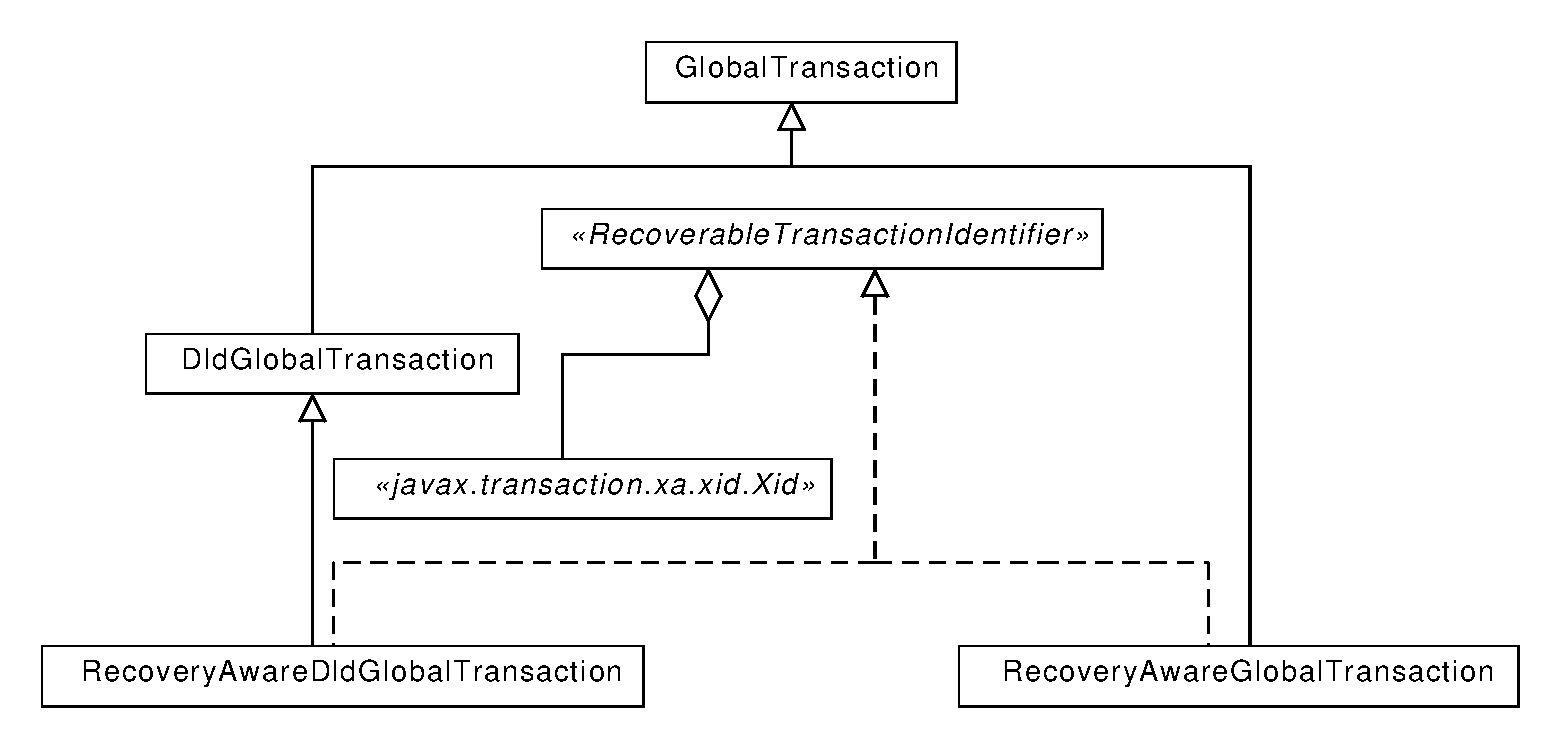
\includegraphics[width=\textwidth]{global_transaction} 
  \caption{GlobalTransaction}
  \label{fig:global_transaction} 
\end{figure}

Os comandos que encapsulam operações diretamente relacionadas a uma transação são PrepareCommand, CommitCommand e RollbackCommand. PrepareCommand registra a transação relacionada na estrutura de dados do Infinispan que controla as transações (TransactionTable). CommitCommand e RollbackCommand marcam nessa mesma tabela que a transação relacionada foi finalizada. Outros compartamentos relacionados à esses comandos são implementados nos interceptadores TxInterceptor e TxDistributionInterceptor. TxInterceptor gerencia os comandos transacionais recebidos de outros nós, e TxDistributionInterceptor distribui comandos dentro da transação (como escrita, leitura, etc) para os nós responsáveis pelas chaves especificadas.

Na Listagem \ref{lst:exemplo_transaction} há um trecho de código que ilustra uma transação que utilizaremos para demonstrar como o Infinispan processa transações. Esse código está incompleto e simplificado por questões de clareza.

\begin{lstlisting}[caption={Transação convencional}, label=lst:exemplo_transaction]
cache.getAdvancedCache().getTransactionManager().begin();
cache.put("CHAVE 1", "VALOR 1");
cache.getAdvancedCache().getTransactionManager().commit();
\end{lstlisting}

A primeira linha instrui o gerenciador de transações (\emph{Transaction Manager}) do JTA a criar uma nova transação (\emph{javax.transaction.Transaction} \cite{jta}) e associá-la com a \emph{thread} de execução atual (\cite{ipc}). 

A segunda linha instrui o cache a inserir um novo elemento. Internamente, a classe CacheImpl irá criar os dois objetos necessários para a execução da operação. Um deles é PutKeyValueCommand, responsável por armazenar na chave especificada o valor fornecido. O outro objeto é LocalTxInvocationContext, que vai representar uma execução transacional iniciada no mesmo nó que executa o comando. 

Após criar o comando e o contexto de execução, o infinispan inicia o processamento do comando, oferecendo a cada interceptador configurado a oportunidade de aplicar sua lógica específica à execução do comando em questão. Os interceptadores mais relevantes na execução do comando de escrita são TxInterceptor, LockingInterceptor e EntryWrappingInterceptor.

TxInterceptor vai criar uma implementação de CacheTransaction e mapeá-la para a Transaction criada pela TransactionManager (associada à thread de execução). Dessa forma, a transação pode ser propagada para outro nós (uma vez que a Transaction do JTA não é propagada) e permite que vários nós executem operações em uma mesma transação. O tipo mais comum de CacheTransaction utilizado é o SyncLocalTransaction, que irá permitir que o TransactionManager notifique o infinispan que uma transação foi finalizada.

LockingInterceptor é responsável por efetuar a trava das chaves relacionadas ao comando. Existem duas implementações desse interceptador: OptimisticLockingInterceptor e PessimisticLockingInterceptor. Optimistic utiliza uma abordagem otimista no processo de travamento, postergando a obtenção da trava para o momento da efetivação da transação. Pessimistic tenta obter as travas no momento da execução do comando.

EntryWrappingInterceptor é responsável por obter as entradas do cache referentes às chaves especificadas no comando e disponibilizá-las no contexto de execução. Essas entradas são encapsuladas por uma classe, MVCCEntry, que permite o multiversionamento dos valores e garante as propriedades ACID da transação.

Por último, CallInterceptor irá executar o método \emph{perform} de PutKeyValueCommand, que por sua vez irá alterar o valor da entrada armazenada no contexto de execução disponibilizado por EntryWrappingInterceptor.

A terceira linha faz com que TransactionManager inicie o processo de efetivação da transação. O infinispan faz uso do mecanismo de notificação de eventos do JTA para ser avisado que a transação foi finalizada. Quando isso acontece, é criado um novo contexto de execução e um novo comando do tipo PrepareCommand. Esse comando representa a primera fase do 2PC, e é responsável por notificar os nós participantes da transação que a transação foi finalizada. 

Esse comando será processado pela mesma cadeia de interceptadores configurada, e os interceptadores mais relevantes para esse execução são TxInterceptor e TxDistributionInterceptor. TxInterceptor fica responsável por registrar como \textbf{preparada} a transação em questão, e TxDistributionInterceptor é o responsável por replicar o comando para os outros nós envolvidos na transação.

O próximo passo dependerá do resultado da execução de PrepareCommand. Se nenhum erro ocorrer, TransactionManager irá então solicitar a efetivação da transação. Caso contrário, a transação será cancelada. No caso de efetivação é criado um CommitCommand e no caso de cancelamento, um RollbackCommand. Os dois comandos resultam em marcar a transação como finalizada, mas CommitCommand faz com que EntryWrappingInterceptor efetive as alterações efetuadas nas entradas, disponibilizando-as para outras transações.

\subsection{Suporte a minitransações}
\label{sec:suporte_mt_infinispan}

O objetivo deste trabalho é implementar uma infraestrutura para o desenvolvimento de sistemas distribuídos baseada em minitransações. Para isso, foram necessárias alterações no código do Infinispan para que esse pudesse suportar a execução de minitransações.

\begin{figure}
  \centering
  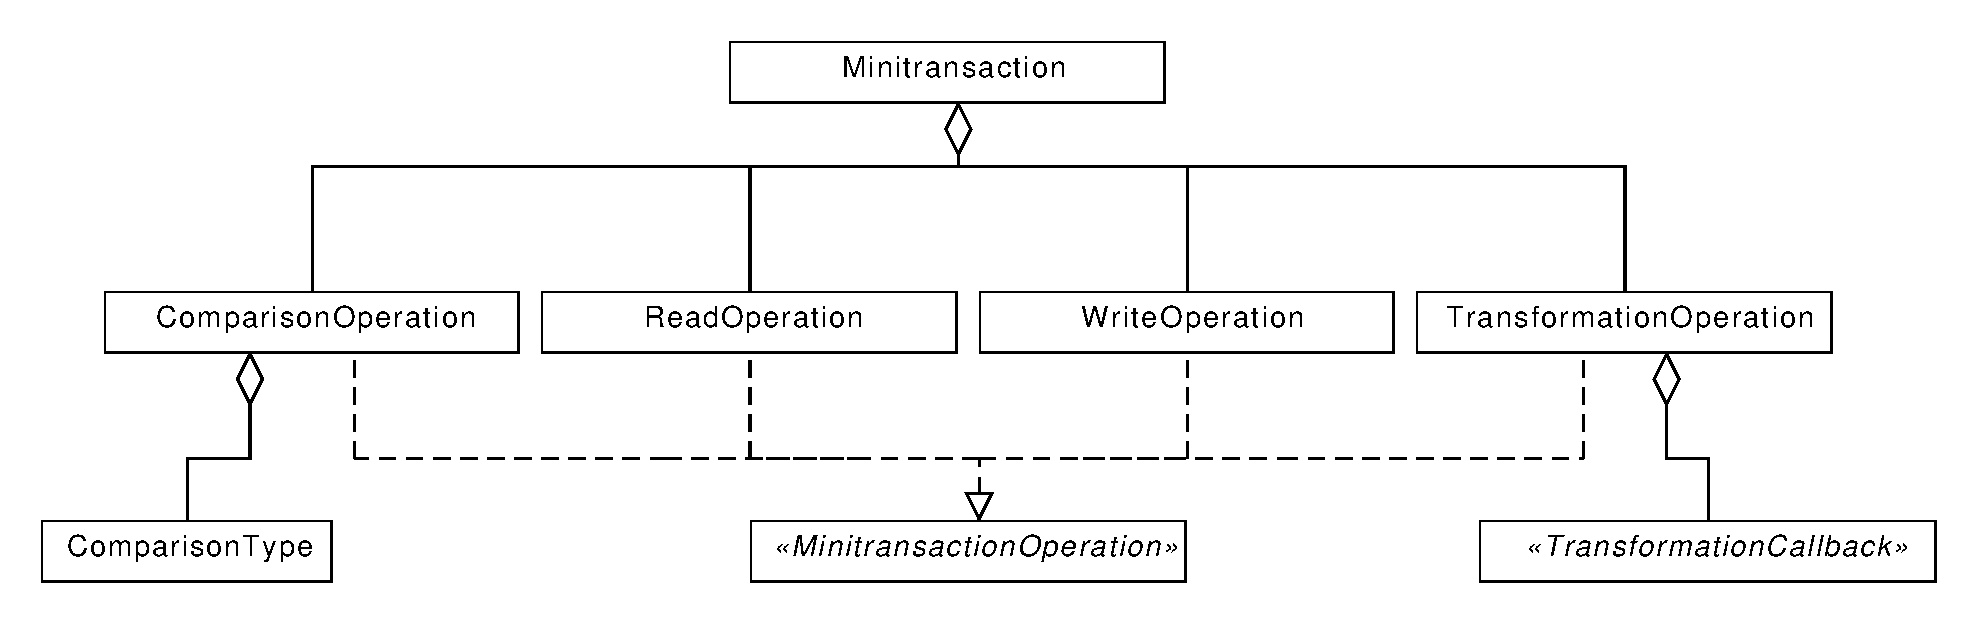
\includegraphics[width=\textwidth]{transaction_operations} 
  \caption{Estrutura de classes das minitransações}
  \label{fig:transaction_operations} 
\end{figure}

A primeira alteração foi a criação de uma estrutura para representar uma minitransação, ilustrada na figura \ref{fig:transaction_operations}. Minitransaction é a classe que agrupa as operações que podem ser efetuadas no contexto de uma minitransação. A interface MinitransactionOperation é a base que deve ser implementada por qualquer operação que faça parte de uma minitransação.

A operação mais simples é ReadOperation, que especifica a chave cujo valor associado deve ser retornado. ComparisonOperation vai efetuar uma comparação, designada por ComparisonType, entre um valor especificado pelo usuário e o valor associado à chave no cache. WriteOperation irá armazenar no cache o valor especificado e associá-lo à chave especificada. TransformationOperation é a operação mais flexível, pois permite que o usuário aplique uma função de transformação no valor associado à chave especificada. Essa função de transformação é uma implementação de TransformationCallback.

A listagem \ref{lst:exemplo_minitransaction} contém código utilizando minitransações com funcionalidade equivalente ao código da listagem \ref{lst:exemplo_transaction}, e apresenta os principais elementos presentes ao codificarmos utilizando minitransações.

\begin{lstlisting}[caption={Minitransação}, label=lst:exemplo_minitransaction]
Minitransaction minitransaction = new Minitransaction();
minitransaction.addWrite(new WriteOperation("CHAVE 1", "VALOR 1"));
MinitransactionExecution execution = cache.getAdvancedCache().execute(minitransaction);
\end{lstlisting}

O método \textbf{execute} de AdvancedCache inicia criando uma transação em TransactionManager. Esse passo é necessário pois a execução de minitransações é baseada no subsistema de transações do infinispan, e esse vai exigir a presença de uma transação no contexto de execução.

Como segundo passo, \textbf{execute} cria uma PrepareMinitransactionCommand, referenciando o objeto Minitransaction recebido como parâmetro. Esse comando percorre então a cadeia de interceptadores, sendo tratado em quase todos eles da mesma maneira que um PrepareCommand, com exceção de TxInterceptor.

O papel de TxInterceptor ao interceptar PrepareMinitransactionCommand é popular a tabela de transações com uma nova CacheTransaction associada à Transaction atual, e associar ao comando a GlobalTransaction que vai permitir que a transação seja identificada dentro do agrupamento, quando o comando for replicado para os outros nós envolvidos.

A lógica de execução da minitransação, descrita na seção \ref{subsec:estrutura-minitransacoes}, é implementada no método \textbf{perform} de PrepareMinitransactionCommand. O nó para o qual a minitransação foi submetida - aquele em que o método \textbf{execute} foi executado - será chamado aqui de coordenador, e os demais nós envolvidos - aqueles responsáveis por chaves envolvidas na minitransação - são chamados de participantes. Devido ao caráter não-centralizado do infinispan, qualquer minitransação pode ser submetida a qualquer nó do agrupamento, inclusive um nó que não seja responsável por nenhuma chave envolvida na minitransação. Uma chave está envolvida na minitransação se ela for referenciada por qualquer operação dessa minitransação.

O objeto Minitransaction que originou a execução é repassado para todos os nós envolvidos, mas cada nó executa somente as operações relacionadas às chaves sob sua responsabilidade. A replicação de dados que não serão usados não acarreta grandes problemas de performance, mas é um ajuste que pode ser feito facilmente no futuro.

A arquitetura do infinispan permite que tanto o código do coordenador quanto dos participantes seja centralizado no método \textbf{perform} do comando. Quando esse comando é executado como resultado da submissão da minitransação para o coordenador, o fluxo é simplesmente um encadeamento de chamadas de métodos dentro da mesma JVM, que culminam na execução de \textbf{perform} (o código completo dessa função foi disponibilizado na listagem \ref{lst:perform}) e na obtenção do resultado dessa execução, um MinitransactionExecution. Quando replicado para os participantes, esse comando é transmitido pela rede, reconstruído em cada participante e inserido no fluxo de execução de comandos, como uma chamada de método comum. O objeto retornado pelo método como resultado de sua execução percorre o caminho inverso, sendo enviado de cada participante de volta para o coordenador.

\begin{lstlisting}[caption={Função PrepareMinitransactionCommand.perform}, label=lst:perform]
@Override
public Object perform(InvocationContext ctx) throws Throwable {

  if( ctx == null ) {
    RemoteTransaction transaction = txTable.getRemoteTransaction(globalTx);

    if (transaction == null) {
      transaction = txTable.createRemoteTransaction(globalTx, null);
    }
         
    ctx = icc.createRemoteTxInvocationContext(transaction, getOrigin());
  }
  
  boolean originLocal = ctx.isOriginLocal();
      
  MinitransactionExecution execution = new MinitransactionExecution();
      
  boolean comparisonResult = true;

  processKeys();
      
  if(!localKeys.isEmpty()) {
    LockControlCommand lockControlCommand = cf.buildLockControlCommand(localKeys, flags, globalTx);
    lockControlCommand.setOrigin(getOrigin());
    invoker.invoke(ctx, lockControlCommand);

    for (ComparisonOperation comparison : minitransaction.getComparisons()) {
      if( localKeys.contains(comparison.getKey()) ) {
        KeyValueComparisonCommand comparisonCommand = cf.buildKeyValueComparisonCommand(comparison, EnumSet.noneOf(Flag.class));
        Object invoke = invoker.invoke(ctx, comparisonCommand);
        if (invoke != null && invoke instanceof Boolean) {
          if (!(comparisonResult = (Boolean) invoke)) {
            break;
          }
        }
      }
    }
  }

  if (!comparisonResult) {
    execution.markAsAborted();
  } else {
    for (ReadOperation read : minitransaction.getReads()) {
      if( localKeys.contains(read.getKey()) ) {
        GetKeyValueCommand getKeyValueCommand = cf.buildGetKeyValueCommand(read.getKey(),
        EnumSet.noneOf(Flag.class));

        Object invoke = invoker.invoke(ctx, getKeyValueCommand);
        execution.addReadKeyValue(read.getKey(), invoke);
      }
    }

    List<WriteCommand> modifications = new ArrayList<WriteCommand>();
    for (WriteOperation write : minitransaction.getWrites()) {
      if( localKeys.contains(write.getKey()) ) {
        PutKeyValueCommand putKeyValueCommand = cf.buildPutKeyValueCommand(write.getKey(), write.getValue(), -1,
               -1, EnumSet.noneOf(Flag.class));
        if(originLocal) {
          invoker.invoke(ctx, putKeyValueCommand);
        }
        else {
          modifications.add(putKeyValueCommand);
        }
      }
    }

    for (TransformationOperation transformation : minitransaction.getTransformations()) {
      if( localKeys.contains(transformation.getKey()) ) {
        TransformCommand transformCommand = cf.buildTransformCommand(transformation.getKey(), transformation.getCallback(), -1,
                -1, EnumSet.noneOf(Flag.class));
        if(originLocal) {
          invoker.invoke(ctx, transformCommand);
        }
        else {
          modifications.add(transformCommand);
        }
      }
    }
         
    if( originLocal ) {
      PrepareMinitransactionCommand remote = new PrepareMinitransactionCommand(cacheName, minitransaction, globalTx);
      remote.setOrigin(rm.getAddress());
      Collection<Address> affectedNodes = new HashSet<Address>(dm.getAffectedNodes(minitransaction.getAllKeys()));
      affectedNodes.remove(rm.getAddress());
      Map<Address, Response> responses = rm.invokeRemotely(affectedNodes, remote, true);
      for( Response response : responses.values() ) {
        if(response.isSuccessful()) {
          SuccessfulResponse sr = (SuccessfulResponse) response;
          MinitransactionExecution remoteExecution = (MinitransactionExecution) sr.getResponseValue();
          execution.mergeWith( remoteExecution );
        }
        else {
          execution.markAsAborted();
        }
        if(execution.isAborted()){
          break;
        }
      }
    }
    else {
      PrepareCommand prepareCommand = cf.buildPrepareCommand(globalTx, modifications, true);
      invoker.invoke(ctx, prepareCommand);
    }
  }

  return execution;
}
\end{lstlisting}

O primeiro passo na execução é obter acesso exclusivo às chaves envolvidas na transação utilizando o mecanismo de travas do infinispan. Um LockControlCommand é criado e executado na cadeia de interceptadores. Se não for possível travar uma ou mais chaves, ocorrerá um erro e a minitransação será cancelada.

Com as entradas referentes às chaves da minitransação travadas, são executadas todas as comparações referentes ao nó atual. Se alguma delas falhar, a minitransação como um todo deve ser cancelada. Para indicar isso, é utilizado o método \textbf{markAsAborted} de MinitransactionExecution. Se todas as comparações forem bem-sucedidas, ou se não houver nenhuma comparação para o nó atual, o fluxo de execução segue.

As operações de leitura são efetuadas em seguida. Para isso, são criados e executados comandos do tipo GetKeyValueCommand, um para cada chave especificada. O valor retornado pela execução de cada um desses comandos é registrado em MinitransactionExecution, com o método \textbf{addReadKeyValue}.

Após as leituras é a vez das operações de escrita, efetuadas com o comando PutKeyValueCommand. Esses comandos são enviados para a cadeia de interceptadores e segue o mesmo fluxo de execução descrito na seção \ref{sec:tx_infinispan}.

O último tipo de operação a ser efetuado é a transformação, que é representada por TransformCommand e por sua implementação de TransformationCallback. Esse comando é semanticalmente muito semelhante à PutKeyValueCommand no sentido em que ele atribui um valor a uma entrada. A diferença é que esse valor é uma função aplicada sobre o valor já existente na entrada. Essa função é representada pela interface TransformCallback e é implementada de acordo com a necessidade do usuário.

Para o nó participante, \textbf{perform} termina nesse ponto, retornando um MinitransactionExecution que será transmitido pela rede para o coordenador. O nó coordenador precisa agrupar todos os resultados obtidos dos participantes e combiná-los por meio do método \textbf{mergeWith} de MinitransactionExecution. Esse método vai agrupar em um só conjunto os resultados das leituras efetuadas e irá marcar esse resultado combinado como sendo cancelado caso algum dos resultados obtidos tenha sido cancelado.

Esse resultado combinado é retornado pelo coordenador e é utilizado pelo método \textbf{execute} para determinar se a minitransação deve ser efetivada ou não. Se \textbf{isAborted} for verdadeiro, a minitransação deve ser abortada e suas alterações devem ser desfeitas. Caso contrário, as alterações devem ser efetivadas e disponibilizadas para futuras transações. Esse processo de efetivação e cancelamento segue o fluxo normal de efetivação e cancelamento do infinispan, sem passar porém pela fazer de preparação do 2PC.

\chapter{Avaliação e resultados}
\label{cap:resultados}

Inicialmente foi pretendido executar os testes baseado na comparação de referências (\emph{benchmarks}), em que os sistemas são executados em um ambiente controlado e os resultados são comparados com valores de referência. O benchmark candidato foi o TPC-E \cite{tpce}, que simula a carga de trabalho em um sistema de processamento de transações de uma correta de valores. A escolha desse benchmark foi a princípio natural, pois ele foi criado pelo TPC (\emph{Transaction Processing Performance Council}, ou conselho de performance de processamento de transações), mas por fim não foi possível utilizá-lo. 

Um dos motivos é que os indicadores de performance desse benchmark são em sua maioria voltados para utilização dos do disco rígido, e nossa infraestrutura mantém todos os dados em memória. O segundo motivo foi a indisponibilidade de versões livres do TPC-E implementados em java. Foi feita uma tentativa de execução da implementação em C++, mas o tempo e o esforço de adequação para conseguir conectar à infraestrutura seria muito grande. Por fim, o TPC é um benchmark bem "pesado", exigindo muita infraestrutura de hardware.

Foram encontrados alguns outros benchmarks, mas nenhum com o peso e critérios do TPC, o que não conferiam a esses um caráter muito confiável. Por fim, foi encontrado o Radargun \cite{radargun}, um arcabouço para o desenvolvimento de benchmarks para caches distribuídos, desenvolvido pelo equipe do próprio infinspan. Infelizmente, o código do radargun estava muito atrelado ao formato de transações convencionais, e a dificuldade para modificá-lo foi semelhante à encontrada no TPC-E. Assim, ele também não pode ser utilizado.

Assim, foi definido então que a avaliação seria baseada em comparações entre transações convencionais e minitransações do próprio infinispan. Como a maior parte do código e estrutura é compartilhado por esses dois mecanismos, essa avaliação é consistente. Foi efetuada uma comparação quantitativa em relação ao tempo de execução e outra avaliação qualitativa em relação à complexidade do código. Os testes simulam dois cenários: a transferência de valores entre contas e um leilão.

No primeiro teste, transferência entre contas, dois parâmetros principais foram definidos: número de contas ($C$) e número de operadores ($O$). Cada conta é identificada por um número entre 1 e $C$, assim como cada operador é identificado por um número entre 1 e $O$. Cada conta recebe um valor inicial uniformemente distribuído no intervalo [1,6]. Cada operador é responsável por tentar efetuar um número de transferências igual a $C^2$, e em cada tentativa são escolhidas de forma aleatória as contas de origem, destino e o valor a ser transferido. Se a conta de origem possuir saldo suficiente, a transferência ocorrerá.

A listagem \ref{lst:operator_account} apresenta o trecho de código dos operadores que efetuam a transferência entre as contas. O operador do tipo TRANSACTION utiliza uma transação convencional, e MINITRANSACTION utiliza uma minitransação. O saldo das contas é armazenado no infinispan como um valor inteiro, na entrada referente à chave que identifica a conta. 

\begin{lstlisting}[caption={Operadores que executam as transferências}, label=lst:operator_account]
private enum Operator {

  TRANSACTION {

    @Override
    void transfer(Node node, long value, String accountToDebit, String accountToCredit) throws Exception {
      node.startTransaction();
      node.lock(accountToDebit, accountToCredit);
      Long fromValue = (Long) node.get(accountToDebit);
      Long toValue = (Long) node.get(accountToCredit);

      if (value <= fromValue) {
        Long newValueOfDebitAccount = fromValue - value;
        Long newValueOfCreditAccount = toValue + value;

        node.put(accountToDebit, newValueOfDebitAccount);
        node.put(accountToCredit, newValueOfCreditAccount);
        node.commitTransaction();
      } else {
        node.rollbackTransaction();
      }
    }

  },
  MINITRANSACTION {

    @Override
    void transfer(Node node, long value, String accountToDebit, String accountToCredit) {
      Minitransaction minitransaction = new Minitransaction();
      minitransaction.addComparison(ComparisonType.GE.create(accountToDebit, value));
      minitransaction.addTransformation(new TransformationOperation(accountToDebit, new AddValue(-value)));
      minitransaction.addTransformation(new TransformationOperation(accountToCredit, new AddValue(value)));
      node.execute(minitransaction);
    }

  };

  abstract void transfer(Node node, long value, String accountToDebit, String accountToCredit) throws Exception;

}
\end{lstlisting}

O segundo teste, leilão, utiliza dois parâmetros também: o número de leilões ($L$) e o número de participantes ($P$). Cada leilão é identificado com um número sequencial entre 1 e $L$, e cada participante é identificado por um número sequencial entre 1 e $P$. O infinispan é utilizando para armazenar o valor do lance vencedor da última rodada de cada leilão e o identificador do participante que efetuou esse lance vencedor.

Cada leilão recebe um valor inicial entre 1 e 6, e cada participante recebe um saldo inicial (o valor de sua carteira, \emph{wallet}) que garante que esse participante consiga efetuar no mínimo um lance. Os participantes tentam efetuar um lance de cada vez, em cada um dos leilões, em sequência, enquanto tiverem saldo em suas carteiras. Um participante não irá tentar um lance se ele já deu o lance mais alto na rodada anterior. A listagem \ref{lst:bidder_auction} apresenta o código dos participantes utilizando um transação convencional (TRANSACTION) e uma minitransação (MINITRANSACTION).  

\begin{lstlisting}[caption={Participante que efetuam os lances}, label=lst:bidder_auction]
private enum Bidder {
  TRANSACTION{

    @Override
    int bid(Node node, int id, Wallet wallet, Auction currentAuction) throws Exception {
      int count = 0;
      node.startTransaction();
      node.lock(currentAuction.code, currentAuction.code + "_WINNER");
      Integer lastBid = (Integer) node.get(currentAuction.code);
      Integer currentWinner = (Integer) node.get(currentAuction.code + "_WINNER");
      if( currentWinner != null && currentWinner == id ) {
        count++;
        node.rollbackTransaction();
      }
      else if( wallet.value <= lastBid ) {
        count++;
        node.rollbackTransaction();
      }
      else {
        int currBid = Math.min(lastBid + 1, wallet.value);
        if( currBid <= lastBid ) {
          node.rollbackTransaction();
        }
        else {
          node.put(currentAuction.code, currBid);
          node.put(currentAuction.code + "_WINNER", id);
                     
          wallet.value -= currBid;
                     
          node.commitTransaction();
        }
      }
      return count;
    } 
  },
  MINITRANSACTION{

    @Override
    int bid(Node node, int id, Wallet wallet, Auction currentAuction) throws Exception {
      int count = 0;
      Minitransaction minitransaction = new Minitransaction();
            
      minitransaction.addComparison(ComparisonType.NE.create(currentAuction.code + "_WINNER", id));
      minitransaction.addComparison(ComparisonType.LT.create(currentAuction.code, wallet));
      minitransaction.addWrite(new WriteOperation(currentAuction.code + "_WINNER", id));
      minitransaction.addTransformation(new TransformationOperation(currentAuction.code, new PlusOne()));
      minitransaction.addRead(new ReadOperation(currentAuction.code));
            
      MinitransactionExecution execution = node.execute(minitransaction);
      if( execution.isAborted() ) {
        count++;
      }
      else {
        wallet.value -= (Integer)execution.get(currentAuction.code) + 1;
      }
            
      return count;
    }
         
  };
      
  abstract int bid(Node node, int id, Wallet wallet, Auction currentAuction ) throws Exception;
}
\end{lstlisting}

Os testes foram executados utilizando o sistema operacional Ubuntu, versão 12.04, com kernel versão 3.5.0-34-generic em dois ambientes distintos. No primeiro ambiente, foi utilizado apenas um computador com processador Intel\textregistered{} Core\texttrademark{} i5 CPU, modelo 480, com 4 núcleos de 2.67GHz e com 6 GB de memória RAM. O segundo ambiente foi composto por duas máquinas virtuais com configurações idênticas ao do primeiro ambiente, em uma Blade HP (*** pegar a configuração).

As tabelas em \ref{tab:tempos_account} apresentam os tempos de execução de diversas configurações do teste que simula as transferências entre contas, quando utilizando transações e minitransações. De maneira semelhante, as tabelas em  \ref{tab:tempos_auction} apresentam os tempos do teste que simula os participantes de um leilão. Os valores estão em segundos, e são médias calculadas dos valores reais de medições obtidas das execuções efetuadas nos ambientes descritos acima.

\begin{table}[h]
	\centering
    	\begin{tabular}{|l|l|l|l|l|l|}
		\hline
		\textbf{Transação} & \multicolumn{5}{l}{No. Operadores} \\
		\hline
		No. Contas & 1 & 2 & 3 & 4 & 5 \\
		\hline
		10 &  &  &  &  &  \\
		\hline
		20 &  &  &  &  &  \\
		\hline
		50 &  &  &  &  &  \\
		\hline
		100 &  &  &  &  &  \\
		\hline
	\end{tabular}
	\begin{tabular}{|l|l|l|l|l|l|}
		\hline
		\textbf{Minitransação} & \multicolumn{5}{l}{No. Operadores} \\
		\hline
		No. Contas & 1 & 2 & 3 & 4 & 5 \\
		\hline
		10 &  &  &  &  &  \\
		\hline
		20 &  &  &  &  &  \\
		\hline
		50 &  &  &  &  &  \\
		\hline
		100 &  &  &  &  &  \\
		\hline
	\end{tabular}
	\caption{Tempos de execução - transferência de valores}
	\label{tab:tempos_account}
\end{table}

\begin{table}[h]
	\centering
    	\begin{tabular}{|l|l|l|l|l|l|}
		\hline
		\textbf{Transação} & \multicolumn{5}{l}{No. Operadores} \\
		\hline
		No. Contas & 1 & 2 & 3 & 4 & 5 \\
		\hline
		10 &  &  &  &  &  \\
		\hline
		20 &  &  &  &  &  \\
		\hline
		50 &  &  &  &  &  \\
		\hline
		100 &  &  &  &  &  \\
		\hline
	\end{tabular}
	\begin{tabular}{|l|l|l|l|l|l|}
		\hline
		\textbf{Minitransação} & \multicolumn{5}{l}{No. Operadores} \\
		\hline
		No. Contas & 1 & 2 & 3 & 4 & 5 \\
		\hline
		10 &  &  &  &  &  \\
		\hline
		20 &  &  &  &  &  \\
		\hline
		50 &  &  &  &  &  \\
		\hline
		100 &  &  &  &  &  \\
		\hline
	\end{tabular}
	\caption{Tempos de execução - leilão}
	\label{tab:tempos_auction}
\end{table}

Como pode ser notado nas tabelas, os tempos de execução das minitransações se mostraram muito superiores aos tempos de execução das transações convencionais. Esse resultado foi contra a intuição inicial de que as minitransações poderiam ocasionar uma melhora no desempenho das aplicações. Isso deve-se às otimizações que o infinispan faz ao executar as transações. 

A principal dessas otimizações, que demonstrou ser a mais relevante para o bom desempenho das transações convencionais, é relacionada à escrita de dados. Ao executar um comando de escrita em um nó A, como PutKeyValueCommand, cuja chave está sob a responsabilidade de um outro nó B, o infinispan não irá efetuar a escrita no nó remoto. O comando será executado localmente, e somente no momento da finalização da transação é que esse comando será enviado para o nó B, dentro de PrepareCommand.

Todos os comandos de escrita são agrupados e enviados de uma só vez em um PrepareCommand, de modo semelhante ao que acontece com as minitransações. A diferença é que ao executar o PrepareCommand no nó remoto, os comandos de escrita agrupados dentro do prepare são executados de uma vez também, aproveitando o fluxo de execução do PrepareCommand. Enquanto na execução da minitransação cada comando de escrita gera um novo PutKeyValueCommand, e cada um desses comandos é executado e processado por toda a cadeia de interceptadores configurado, no caso do PrepareCommand, não há a criação desses novos comandos de escrita, e a cadeia de interceptadores é percorrida somente uma vez.

Os resultados obtidos não foram satisfatórios mas, como será apresentado na seção \ref{sec:licoes_e_futuro} a seguir, há possibilidade de alterações para melhorar o desempenho do sistema em relação ao desempenho apresentado por transações convencionais. De certa forma, analisando por um ponto de vista quantitativo, este trabalho não atingiu seus objetivos.

Sob uma ótica qualitativa, porém, acreditamos que o trabalho tenha tido êxito. Se compararmos o código das aplicações apresentadas nas listagens anteriores, vemos que os trechos que fazem uso de minitransações são menores e mais claros. É evidente que um menor número de linhas de código não se traduza automaticamente em qualidade mas, nos cenários em que pode ser utilizada, uma minitransação permite expressar de forma mais concisa a intenção da transação.

Por exemplo, nas linhas 12-21 da listagem \ref{lst:operator_account} vemos que o código cliente fica a cargo de cancelar a transação caso a comparação de valores não seja bem sucedida. A intenção da transação fica perdida em meio aos mecanismos que o sistema de transações oferece para utilizá-las. 

Nas minitransações, essa intenção fica clara e não espalhada pelo código. Os aspectos semânticos ficam bem definidos no código: basta verificar as comparações que a minitransação possui para verificar em quais cenários ela será efetivada ou cancelada. Com o uso de transações convencionais, esse aspecto semântico é mais difícil de ser diretamente detectado, exigindo uma análise mais cuidadosa.

Em concordância com uma abordagem de código limpo e claro como uma ferramenta e um meio de desenvolver sistemas de qualidade (\cite{clean_code}, \cite{xp}, \cite{refactoring}), principalmente na área de sistemas distribuídos, onde há um número enorme de cenários não-triviais a serem tratados, a possibilidade de utilizar uma primitiva que traduza claramente a semântica de uma transação que pode envolver uma grande quantidade de máquinas é de grande valor.

\chapter{Conclusão}
\label{cap:conclusao}

Embora tenha sido planejado para ser modificado, houve alguns pequenos problemas para alterar o infinispan para executar minitransações. Esses problemas e as soluções encontradas estão descritos na seção \ref{sec:problemas_solucoes}. Os resultados obtidos com esse trabalho foram disponibilizados para amplo acesso, e uma análise está disponível na seção \ref{sec:resultados}. Na seção \ref{sec:licoes_e_futuro} apresentamos lições aprendidas no desenvolvimento deste trabalho e identificamos pontos que podem ser melhorados, e possíveis extensões.

\section{Problemas e soluções}
\label{sec:problemas_solucoes}

O principal problema encontrado, e de certa forma ainda não resolvido, está relacionado à avaliação da infraestrutura. Esse problema direcionou o desenvolvimento do trabalho para sua direção atual. Os outros problemas estão relacionados ao desenvolvimento.

Inicialmente, foi desenvolvida uma infraestrutura nova, sem utilizar nenhum código como base, em que o processamento de minitransações estava diretamente embutido no sistema. Essa infraestrutura armazena os dados em memória e oferece uma interface de acesso muito parecida à do infinispan. Embora essa primeira infraestrutura desenvolvida funcione e execute minitransações, foram encontrados alguns empecilhos para avaliá-la.

Em primeiro lugar, não foi encontrado nenhum outro sistema que oferecesse essa funcionalidade de execução de minitransações. Não há sentido em avaliar a infraestrutura isoladamente, pois não há nenhum parâmetro de comparação. A avaliação isolada foi feita mas com caráter funcional, para garantir que a infraestrutura estava de acordo com a especificação proposta e que era possível utilizá-la.

A avaliação pretendida era a comparação dos resultados de performance apresentados pela infraestrutura com outros resultados conhecidos, uma vez que um objetivo indireto desse trabalho é demonstrar a efetividade de minitransações como uma alternativa viável para o desenvolvimento de aplicações distribuídas. Porém, essa análise se mostrou mais complexa do que o esperado, pois os outros sistemas disponíveis com funcionalidades semelhantes já estavam consolidados e testados em ambientes de produção de alta-carga, em alguns casos com anos acumulados em melhorias de performance e desempenho.

Surgiu então a idéia de modificar um sistema já existente, que tivesse funcionalidades semelhantes, de forma que a diferença fosse mínima na implementação dos cenários testados. Após a avaliação de alguns candidatos foi escolhido o Infinispan, pois apresentava a maioria das características desejadas para a infraestrutura e era desenvolvido em Java, linguagem com a qual o autor deste trabalho possui maior experiência.

Iniciou-se um novo esforço de aprendizagem, pois o Infinispan é um sistema complexo, com muitas funcionalidade e altamente configurável. Seu código é bem estruturado e faz uso de diversos padrões, convenções e boas práticas utilizadas no desenvolvimento de sistemas distribuídos, mas mesmo assim não é de nenhuma forma um código simples. Foram necessárias diversas execuções, novas linhas de log e muitas sessões de debug para que fossem idêntificados os pontos que precisavam ser alterados. 

Ao estender o infinispan, nossa infraestrutura herdou toda sua funcionalidade, como a replicação e distribuição de dados e capacidade de armazenar os dados em diversas formas de armazenagem, como discos ou bancos de dados. Toda a camada de comunição intra-nós e entre a infraestrutura e os clientes também foi reaproveitada. De certa forma, o ponto principal do trabalho passou a ser permitir que o infinispan executasse minitransações, utilizando seus componentes. Isso, porém, não foi tão simples como esperado.

O infinispan pode atuar tanto no modo transacional quanto não-transacional. Porém, o termo "não-transacional" pode dar a impressão de que não há transações envolvidas, o que não é verdade. O deixa de existir é a transação do JTA e a possibilidade de agrupar operações em uma grande operação lógica, demarcada pela usuário. No modo não-transacional, cada operação individual é envolvida por uma transação, criada antes logo no início da execução do comando e finalizada após o fim de sua execução.

Dessa forma, o conceito de transação permeia particamente todo o infinispan, mesmo em trechos que seriam "não-transacionais". Isso dificultou um pouco a inclusão de suporte a minitransações. Por exemplo, não foi possível fazer com que PrepareMinitransactionCommand fosse uma subclasse de PrepareCommand. Inicialmente havia sido codificado dessa forma, mas havia muitos pontos em que PrepareCommand era tratado e a maioria desses pontos não fazia sentido para uma minitransação.

Um outro problema é que o Infinispan faz uma série de otimizações em relação a transações. Uma delas é tratar uma transação distribuída como sendo de somente uma fase, ou seja, em alguns cenários específicos, que dependem da configuração especificada, o infinispan efetua a efetivação ou cancelamento quando processa PrepareCommand. A configuração necessária para habilitar as minitransações resultavam necessariamente nesses cenários, o que atrapalhava a execução das minitransações.

Foram testadas algumas alternativas para a implementação, mas a solução final acabou sendo a mais simples, apresentada no capítulo sobre a implementação da infraestrutura, na seção \ref{sec:suporte_mt_infinispan}. Com essa solução a execução das minitransações ficou desvinculada da maior parte da execução de transações convencionais no infinispan.

O último problema, que remete ao primeiro citado no início dessa sessão foi a escolha de uma ferramenta que possibilitasse a correta medição de parâmetros para uma análise de performance consistente. Devido à diferença estrutural dos tratamentos no código entre transações e minitransações, instrumentar o código para efetuar essas medições não seria muito efetivo.



%5 Threads - AccountTest

%\begin{description}
%	\item[OrdinaryDebtor] 519.653s
%	\item[MinitransactionDebtor] 36000.656s 
%\end{description}

%Foi necessário

%A própria natureza das minitransações dificulta essa comparação pois como vimos, ela está restrita a alguns tipos de operações, sendo menos genérica do que uma transação convencional. Assim, comparar 


%A prosposta deste trabalho é disponibilizar uma infraestrutura com suporte a minitransações para facilitar o desenvolvimento de aplicações distribuídas, mas não foi encontrado nenhum outro sistema que oferecesse essa funcionalidade.



% Nesse âmbito, não foi encontrado nenhum outro sistema que oferecesse essa capacidade específica de minitransações e portanto, foi é possível compará-lo

%Grande parte do esforço de desenvolvimento foi voltado a entender a base de código do infinispan. O seu código está em sua grande maioria bem estruturado, com cada classes com suas responsabilidades bem definidas. A arquitetura da aplicação também foi bem planejada, e a maneira como conceitos e padrões foram usados para viabilizar a complexa tarefa de esconder uma estrutura de cache distribuída atrás de uma interface amigável ao usuário é uma lição muito importante aprendida.


%A primeira proposta desse trabalho era desenvolver uma infraestrutura totalmente do zero, e dessa forma todo o processamento de minitransações estaria embutido no sistema. Esse sistema chegou a ser desenvolvido e, apesar de ter funcionalidades bem simplificadas, as minitransações eram executadas corretamente e de modo integral, mas ele foi descontinuado por apresentar algumas dificuldades com relação à avaliação do sistema.

%A idéia para avaliar o sistema era de comparar  

%Um empecilho ao uso desse sistema era como compará-lo com outros sistemas. Não foi encontrado nenhum outro sistema com suporte a minitransações, e comp

\section{Lições aprendidas e trabalhos futuros}
\label{sec:licoes_e_futuro}

O sistema desenvolvido inicialmente não utilizou nenhum outro código como base. Por esse motivo, foi necessário o desenvolvimento de funcionalidades em áreas diversas, algumas das quais o autor não possuía muita experiência.

A primeira dessas funcionalidades foi a criação de um protocolo para a comunicação e o desenvolvimento de um interpretador para esse protocolo. Mesmo sendo um protocolo simples (esse protocolo foi descrito na versão original do texto de qualificação deste trabalho) o desenvolvimento de um interpretador não é trivial, e exigiu um estudo mais aprofundado das técnicas de construção de interpretadores (disponíveis em \cite{compilers}).

A implementação do gerenciamento e comunicação de rede também não foi simples, pois a comunicação poderia ocorrer tanto entre os nós do sistema quanto entre aplicações clientes e o sistema. Projetado para ser acessível a qualquer aplicação com acesso à uma rede de computador, foi escrito código para lidar direto com a camada \emph{TCP} da rede, utilizando as funcionalidades de entrada e saída não-bloqueantes da plataforma java (\cite{nio}), algo que o autor não havia utilizado de forma consistente anteriormente.

Esse primeiro sistema, embora tenha chegado a um estágio funcional, ficou longe de estar completo, e as funcionalidades descritas acima, vitais para a execução do sistema, também eram incompletas e sujeitas a falhas muitas vezes grosseiras. A principal lição aprendida com esse sistema foi buscar e tentar reaproveitar algo que funcione e que possa ser modificado para nossas necessidades, mesmo que tenhamos que nos desfazer de longas horas de trabalho já efetuado.

O uso do infinispan como base exigiu um novo esforço de aprendizado e descoberta. Todas as funcionalidades disponíveis no primeiro sistema, de forma bem mais completa, estavam presentes no infinispan, além de um grande número de outras que apesar de importantes, não seriam desenvolvidas por falta de tempo.

Estudar e entender a base de código do infinispan agregou muito em termos de como desenvolver um sistema totalmente distribuído, capaz de executar em diversos cenários, muitos dos quais não haviam sequer sido cogitados na proposta deste trabalho. Foi importante ver também que o próprio infinispan foi construído com base em outras sólidas bases, como o JGroups, e como muitos dos problemas enfrentados no desenvolvimento do primeiro sistema não causariam impacto se esse biblioteca tivesse sido utilizada.

Como descrito anteriormente, uma pendência deste trabalho é a otimização da execução da minitransação para melhorar seu desempenho em relação ao tempo de execução das transações convencionais. Poderia ser criado somente um comando para executar todas as escritas de uma vez, como é feito no caso do PrepareCommand, evitando assim que a cadeia de interceptadores seja percorrida repetidamente.

Uma segunda oportunidade de desenvolvimento é a validação e execução dos testes em um ambiente altamente distribuído. Conforme descrito na descrição do infinispan e baseado em discussões dos desenvolvedore do infinispan, foi reportado a utilização de agrupamentos do infinispan contendo 400 máquinas, mas as configurações para esses agrupamentos não foram divulgadas. 

De forma mais realista, a documentação do infinispan descreve como configurar e otimizar para agrupamentos de até 128 máquinas. Executar e analisar o comportamento das minitransações, uma vez que seus problemas de performance sejam corrigidos, em um ambiente com essas configurações seria muito interessante. 

Por fim, a separação de uma definição de minitransação de suas implementações parece uma proposta promissora, nos moldes do que acontece com as transações convencionais e o JTA. Como visto na seção \ref{sec:resultados}, o uso de uma minitransação permite uma representação mais direta das intenções da transação, o que pode torná-las uma ferramenta para auxiliar no desenvolvimento de um código mais claro e coeso, independente do sistema ser distribuído ou não.

% cabeçalho para os apêndices
%\newpage
%\renewcommand{\chaptermark}[1]{\markboth{\MakeUppercase{\appendixname\ \thechapter}} {\MakeUppercase{#1}} }
%\fancyhead[RE,LO]{}
%\appendix
%\chapter{Códigos}

%Esse apêndice apresenta algumas listagens mais completas de códigos e exemplos de utilização do infinispan.

%\label{apx:codigo}

% ---------------------------------------------------------------------------- %
\backmatter \singlespacing   % espaçamento simples
\bibliographystyle{alpha-ime}% citação bibliográfica alpha
\bibliography{bibliografia}  % associado ao arquivo: 'bibliografia.bib'

\end{document}
